% !TEX encoding = UTF-8 Unicode
% !TEX root = SystemTemplate.tex

\documentclass{book}

% !TEX root = SystemTemplate.tex

\usepackage[width=6.5in, height=9.2in, top=1.0in, papersize={8.5in,11in}]{geometry}
\usepackage[pdftex]{graphicx}
\usepackage{amsmath}
\usepackage{amsthm}
\usepackage{amssymb}
%\usepackage{txfonts}
\usepackage{textcomp}
\usepackage{amsthm}

\usepackage[all]{xy}
\usepackage{fancyhdr}
\pagestyle{fancy}
\usepackage{hyperref}
\usepackage{verbatim}
\usepackage{algorithm}
\usepackage{algorithmic}
\usepackage{array}
\usepackage{color}
\usepackage{listings}
\usepackage{calc}
\usepackage{doxygen}
\usepackage[utf8]{inputenc}
\usepackage{makeidx}
\usepackage{multicol}
\usepackage{multirow}
\usepackage[table]{xcolor}
\usepackage{tabularx}
\usepackage{framed}
\usepackage{xspace}
\usepackage{etex}
\usepackage{todonotes}
\usepackage{pdfpages}
\usepackage{pgfgantt}


%% Computer Modern Bright Font
%\usepackage{cmbright}
%\usepackage[T1]{fontenc}

%% Sans Serif Modern Font - similar to  Helvetica
\usepackage{lmodern}
\renewcommand*\familydefault{\sfdefault} %% Only if the base font of the document is to be sans serif
\usepackage[T1]{fontenc}


\definecolor{SDColor1}{rgb}{0,0,0}
\definecolor{SDColor2}{rgb}{0,0,0}
\definecolor{SDColor3}{rgb}{0,0,0}
\definecolor{SDColor4}{rgb}{0,0,0}
\definecolor{SDColor5}{rgb}{0,0,0}

%%%  --- Here are some other colors.  Keep it conservative --- %%%

%% Blue font color scheme
%\definecolor{SDColor1}{rgb}{.204,.353,.541}
%\definecolor{SDColor2}{rgb}{.31,.506,.741}
%\definecolor{SDColor3}{rgb}{0.18,0.35,0.59}
%\definecolor{SDColor4}{rgb}{0.44,0.59,0.82}
%\definecolor{SDColor5}{rgb}{0.35,0.35,0.35}
%

%% Brown color scheme
% \definecolor{SDColor1}{rgb}{.55,.2,.2}
%\definecolor{SDColor2}{rgb}{.4,.1,.1}
%\definecolor{SDColor3}{rgb}{.5, .15,.15}
%\definecolor{SDColor4}{rgb}{.63,.32,.18}
%\definecolor{SDColor5}{rgb}{.45,.15,.15}
%


%% Custom colors for code listing environment
\definecolor{OliveGreen}{cmyk}{0.64,0,0.95,0.40}
\definecolor{DarkBlue}{cmyk}{0.76,0.76,0,0.20}
\definecolor{DarkRed}{cmyk}{0,1,1,0.45}
\lstset{language=c,frame=ltrb,framesep=5pt,basicstyle=\normalsize,
 keywordstyle=\ttfamily\color{DarkRed},
identifierstyle=\ttfamily\color{DarkBlue}\bfseries,
commentstyle=\color{OliveGreen},
stringstyle=\ttfamily,
showstringspaces=false,tabsize = 3}


\setlength{\oddsidemargin}{0mm} 
\setlength{\evensidemargin}{0mm} 

%% Uncomment if you want "Draft" placed on each page.
%\usepackage{draftwatermark}
%\SetWatermarkLightness{0.975}
%\SetWatermarkScale{1}
%\SetWatermarkText{Draft}

\pagestyle{fancy}
\renewcommand{\chaptermark}[1]{\markboth{#1}{}}
\renewcommand{\sectionmark}[1]{\markright{\thesection\ #1}}
\fancyhf{}
\fancyhead[LE,RO]{\bfseries\thepage}
\fancyhead[LO]{\bfseries\rightmark}
\fancyhead[RE]{\bfseries\leftmark}
%\fancyfoot[LE,RO]{Confidential and Proprietary}
%\renewcommand{\headrulewidth}{0.5pt}
%\renewcommand{\footrulewidth}{0pt}
%\addtolength{\headheight}{0.5pt}
%\setlength{\footskip}{0mm}
%\renewcommand{\footruleskip}{0pt}



\usepackage{titlesec}
\titleformat{\chapter}[display]
{\normalfont\bfseries\color{SDColor3}}    %\normalfont\bfseries\filcenter}
{\LARGE\thechapter}
{1ex}
{\titlerule[2pt]
\vspace{2ex}%
\LARGE}
[\vspace{1ex}%
{\titlerule[2pt]}]

%
%\usepackage{titlesec}
%\titleformat{\chapter}{\normalfont\bfseries\LARGE}
%{\thechapter.}{5pt}{}[{\titlerule[3pt]}]
%
%\titleformat{\section}{\normalfont\bfseries\Large}
%{\thesection.}{5pt}{}[{\titlerule[2pt]}]
%
%\titleformat{\subsection}{\normalfont\bfseries\large}
%{\thesubsection.}{5pt}{}[{\titlerule[1pt]}]
%


%\titleformat*{\section}{\Large\bfseries\sffamily\color{SDColor1}}
%\titleformat*{\subsection}{\large\bfseries\sffamily\color{MSLightBlue}}
%\titleformat*{\section}{\Large\bfseries\color{SDColor3}}
%\titleformat*{\subsection}{\large\bfseries\color{SDColor4}}

%\titleformat*{\section}{\Large\bfseries}
%\titleformat*{\subsection}{\large\bfseries}
%\titleformat*{\subsubsection}{\large\bfseries}

\titleformat*{\section}{\Large\bfseries\color{SDColor1}}  
\titleformat*{\subsection}{\large\bfseries\color{SDColor2}}
\titleformat*{\subsubsection}{\large\bfseries\color{SDColor5}}
\setcounter{secnumdepth}{3}
\renewcommand{\thesubsubsection}{\thesubsection.\alph{subsubsection}}

% Save the original chapter command as stdchapter
\let\stdchapter\chapter

%redefine the backmatter command
\let\stdbackmatter\backmatter
\makeatletter% We need the '@' letter to call if@openright
\renewcommand{\backmatter}{
\stdbackmatter
% need to set the page counter back to 1
\setcounter{page}{1}
%% Redefine the \chapter command for our Back Matter
\renewcommand{\chapter}[1]{
  \if@openright\cleardoublepage\else\clearpage\fi% chapters begin on right page
  \stdchapter{##1}% output standard chapter heading
  \setcounter{section}{0}% restart the section numbering
  \renewcommand{\thepage}{BM-\arabic{page}}% Redefine page numbering format
  \renewcommand{\thesection}{\arabic{section}}% Redefine section number format
}}
\makeatother% Restore the normal behavior of '@'

%redefine the appendix command
\let\stdappendix\appendix
\makeatletter% We need the '@' letter to call if@openright
\renewcommand{\appendix}{
\stdappendix
%% \titleformat{\chapter}[display]
%% {\normalfont\bfseries\color{SDColor3}}    %\normalfont\bfseries\filcenter}
%% {\LARGE Appendix \thechapter}
%% {1ex}
%% {\titlerule[2pt]
%% \vspace{2ex}%
%% \LARGE}
%% [\vspace{1ex}%
%% {\titlerule[2pt]}]
  %%% Since counters are different in the appendix section
  %%% we redefine \chapter to explicitly reset the page number
  %%%  (comment out to see effect)
  \renewcommand{\chapter}[1]{
    \stdchapter{##1}\setcounter{page}{1}
    %%% We also redefine page numbering
    \renewcommand{\thepage}{\Alph{chapter}-\arabic{page}}
  }
}
\makeatother% Restore the normal behavior of '@'


\makeatletter% We need the '@' letter to call if@openright
\newcommand{\agreement}{
  \renewcommand{\chapter}[1]{
    \if@openright\cleardoublepage\else\clearpage\fi% chapters begin on right page
    \pagestyle{plain}% turn off fancy headers
    \setcounter{section}{0}% Reset the section number
    \setcounter{page}{1}% Reset the page number
    \renewcommand{\thepage}{SA-\arabic{page}}% Set format for page numbering
    \renewcommand{\thesection}{\arabic{section}}% Set format for section numbering
    \refstepcounter{chapter}% Add it to the index/toc for on-line viewing
    \addcontentsline{toc}{chapter}{##1}% Add to the table of contents
  }
}
\makeatother% Restore the normal behavior of '@'



%%  If you do some math typesetting, you may want more environment names.
%% Uncomment to see how this works:
%\newtheorem{summary}{Summary:}
%\newtheorem{example}{Example:}



 % This sets the format.

% Add your title page contents here 
\title{{\color{MSBlue1} \rule{\linewidth}{0.5mm}}\\[2mm] {\huge \bfseries \color{MSBlue1} DanceSoft }\\[-1mm] {\color{MSBlue1}\rule{\linewidth}{0.5mm}} \\  \vfill
{\LARGE \bfseries \color{MSBlue2} Senior Design Final Documentation }\\  \vfill 
{\color{MSBlue1} DanceSoft} }
\author{\color{MSBlue1}  Marcus Berger \and \color{MSBlue1} Dicheng Wu}
\date{\color{MSBlue1} \today}


\begin{document}

\frontmatter

\addcontentsline{toc}{chapter}{Title}
\maketitle
\tableofcontents
\addcontentsline{toc}{chapter}{Contents}
\listoffigures
\addcontentsline{toc}{chapter}{List of Figures}
\listoftables
\addcontentsline{toc}{chapter}{List of Tables}
\listofalgorithms
\addcontentsline{toc}{chapter}{List of Algorithms}

\chapter{Overview Statements}
% !TEX root = DesignDocument.tex

\section{Mission Statement}
The mission of the DanceSoft team is to create a efficient and effective system for the Academy of Dance Arts. So data can be managed clearly and easily to manage the academy's day to day needs. [MB]

\section{Elevator Pitch}
The DanceSoft project is a data management software for the Academy of Dance Arts in Rapid City. The project aims to produce a simple and more effective data management tool then what is currently in use at the academy. This will be accomplished through the use of a database and a simple user friendly interface, which will allow faculty and students to easily accomplish their needs, whether that's registering for a class, getting a role sheet or just general people management. DanceSoft will provide effective management tools so people spend less time at their computer, and more time dancing. [MB]  
  % add mission statement to mission.tex

\chapter{Document Preparation and Updates}
% !TEX root = SystemTemplate.tex



Current Version [X.X.X]
\vspace*{5mm}

{\color{MSBlue3}
\noindent
\textit{Prepared By:}\\
\textit{Marcus Berger \#1}\\
\textit{Dicheng Wu \#2}\\
}

\vfill
\noindent
{\color{color02} \textit{\textbf{Revision History}}}\\
\begin{tabular}{|>{\raggedright}p{1.5cm}|>{\raggedright}p{3cm}|>{\raggedright}p{1.5cm}|>{\raggedright}p{9cm}|}
\hline
\textit{\textbf{Date}} &  \textit{\textbf{Author}} & \textit{\textbf{Version}} & \textit{\textbf{Comments}}\tabularnewline
\hline
 \textit{\textbf{9/12/15}} & \textit{Marcus Berger and Dicheng Wu} & \textit{1.0.0} & \textit{Initial version}\tabularnewline
\hline
\textit{\textbf{10/8/15}} & \textit{Marcus Berger} & \textit{1.0.1} & \textit{Sprint Report 1}\tabularnewline
\hline
\textit{\textbf{10/22/15}} & \textit{Marcus Berger} & \textit{1.0.1} & \textit{Initial Overview}\tabularnewline
\hline
\textit{\textbf{10/23/15}} & \textit{Marcus Berger} & \textit{1.0.1} & \textit{Initial Mission Statement and project.tex}\tabularnewline
\hline
\textit{\textbf{10/28/15}} & \textit{Marcus Berger} & \textit{1.0.1} & \textit{Initial Requirements, Testing, and develop.tex }\tabularnewline
\hline
\textit{\textbf{11/5/15}} & \textit{Marcus Berger and Dicheng Wu} & \textit{1.0.2} & \textit{Sprint Report 2}\tabularnewline
\hline
\textit{\textbf{11/5/15}} & \textit{Marcus Berger} & \textit{1.0.2} & \textit{Updated Overview}\tabularnewline
\hline
\textit{\textbf{12/4/15}} & \textit{Marcus Berger and Dicheng Wu} & \textit{1.0.3} & \textit{Sprint Report 3}\tabularnewline
\hline
\textit{\textbf{12/8/15}} & \textit{Marcus Berger} & \textit{1.0.3} & \textit{Updated Project, Uploaded Resume, and Add Acknowledgments}\tabularnewline
\hline
\textit{\textbf{12/9/15}} & \textit{Marcus Berger} & \textit{1.0.3} & \textit{Updated Requirements (future user stories marked with update time frame) }\tabularnewline
\hline
\textit{\textbf{12/9/15}} & \textit{Dicheng Wu} & \textit{1.0.3} & \textit{Uploaded Resume}\tabularnewline
\hline
\textit{\textbf{12/9/15}} & \textit{Marcus Berger} & \textit{1.0.3} & \textit{Minor Update to Testing}\tabularnewline
\hline
 &  &  & \tabularnewline
 \hline
 &  &  & \tabularnewline
\hline
 &  &  & \tabularnewline
\hline
 &  &  & \tabularnewline
\hline
 &  &  & \tabularnewline
\hline
\end{tabular}
\vfill


 
\mainmatter

%%  Add to the following chapters

% !TEX root = SystemTemplate.tex

\chapter{Overview and concept of operations}

This chapter contains a  general overview of the DanceSoft project.


\section{Scope}
This section contain a general explanation of the purpose, deliverables/major components, and goals of the project.


\section{Purpose}
This project is for the Academy of Dance Arts. The project is intended to provide a simple way manage students, employees, classes and manage the day to day activities of the academy . This is done using a database back-end and a PyQt GUI front end. The system will allow teachers to manage their classes, and some student info. Students will be able to register for classes and view their information. System admins such as the owner of the academy can manage all academy data, assign teachers and compute payroll and billing depending on the needs of a specific member of the academy.  

\section{Deliverables} 

\subsection{Major System Component: Database}
The first major component of the system is the MySQL relational database. The database will contain the Academy's data and be the core of the back-end side of the software, and be the conduit for most of the systems interactions with the data. The database will live within a local computer provided by the user.  

\subsection{Major System Component: User Interface}
The second major component of the system is the front-end user interface. This will be the only part of the system most users ever see, and will provide an effective means to complete the desired user task. This is accomplished through the use of pages created in PyQt with interfaces to give users effective ways to interact with the database and the necessary data for their requested operation.

\subsection{Major System Component \#3}
Describe briefly the role this major component plays in this system. 

\section{Systems Goals}
The system needs to provide a solution which can run the dance studio data and some day to day activities in an effective and secure manner. This includes allowing teachers to print role sheets, look at schedules, and manage their information. Students need to have the ability to see information pertinent to them such as registration and class requirements. Owners need to be able to use the system to manage their employees, the academy's students and it classes, and other administrative duties such as billing and payroll  Lastly this system as a whole also needs to be an improvement on the current system in use by the customer and provide an easier and more efficient way to run the clients business.

Overall the system goal is to provide a environment where academy owners, teachers, and students can effectively manage their personal needs and requirements for academy participation and continued operations.


\section{System Overview and Diagram}
Provide a more detailed description of the major system components
without getting too detailed.  This section should contain a
high-level block and/or flow diagram of the system highlighting the
major components.  See Figure~\ref{systemdiagram}.  This is a floating
figure environment.  \LaTeX\ will try to put it close to where it was
typeset but will not allow the figure to be split if moving it can not
happen.  Figures, tables, algorithms and many other floating
environments are automatically numbered and placed in the appropriate
type of table of contents.  You can move these and the numbers will
update correctly.

\begin{figure}[tbh]
\begin{center}
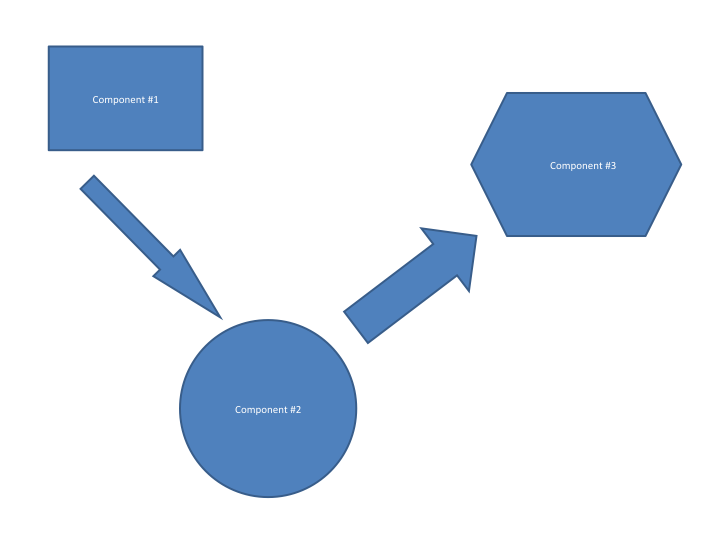
\includegraphics[width=0.75\textwidth]{./diagram}
\end{center}
\caption{A sample figure .... System Diagram \label{systemdiagram}}
\end{figure}

\section{Technologies Overview}
The primary Technologies for this projects are as follows:

\begin{enumerate}
\item Xcode and Visual Studio - Xcode and MSVS are the primary development IDEs for this project. Of the two the one the group used the most was visual studio so we could develop on the machines provided by the school.
\item Python - the primary programming language for the project
\item PHP - primary language for student web interface
\item PyQt and Qt Designer - Gui package and development environment 
\item MySQL - MySQL provides the database and relational quires to manage the data and organize it within the system.
\end{enumerate}


These technologies were selected after a first research sprint where research into programming language, GUI, and database options were selected. A brief description                    of the research can be found in the sprint 1 report or the first prototype sections of this document.  %% All tracks
% !TEX root = SystemTemplate.tex


\chapter{Project Overview}
This section provides some information with regards to the 
team roles, project management, and phase overview.[MB]

\section{Team Members and Roles}
The DanceSoft team consist of two members, Marcus Berger and Dicheng Wu.

Marcus Berger(Scrum Master/Development Team) -  As a member of a two person team the roles for this project blend together significantly. Both team members mostly do equal shares of all work types. As the primary manager of the DanceSoft Trello board, Marcus has mostly taken on the role of scrum master within the group. However his primary role is still development.

Dicheng Wu(Development Team) - Dicheng's primary role as with both members of the team, is development of the software. However like the other members since the team is so small each member of the two person team must be able to fill all needed roles within the team.

Dr. Jeff Mcgough(Product Owner) - While not a working member of the team Dr. Mcgough is a secondary scrum master and product owner to the group due the small size of the team. Main duties in this role include talking to the client about what is needed, and making sure the team stays on task and is going in the correct direction based on the clients needs 

Author notation will be identified by [MB] for Marcus and [DW] for Dicheng at the start of
major sections (ex: after heading 2.0 above). Subsections within the main sections assumed to be by the
same author. [MB]



\section{Project  Management Approach}
This project is managed using several service and an Agile sprint based methodology. The sprints which range in purpose from research to development are three weeks long with a week after each sprint for review and possible presentations to the client. The project is broken into several users stories, which are then broken down into a project backlog of task for development. The stories and backlog are discussed  in a later section of this document. 
Project management tools used by the team are Github, for source control and code management, and Trello for sprint and backlog management. Trello provide a list of task to be accomplished in each sprint and the ability to see modified tasks and keep track of team members current assignments. The task assign in each sprint are decided be the team with some input from Dr. McGough as a secondary scrum master. These assignment can be altered or changed based on product owner input. Sprint reports are sent to Dr. McGough for both project owner and grading purposes at the end of each sprint.
Scheduled Meeting occur every Tuesday and Thursday from 10:00-12:00, other times are assigned as the team finds necessary. The team also has a weekly meeting with the product owner Dr. Jeff McGough every Wednesday at 2:00 where the progress of the project, the next steps, and any lingering questions about the project can be addressed. [MB]


\section{Phase  Overview}
This project will be implemented in phases, the phases follow. [MB]

\subsection{Initial User Story and Requirements Gathering}
This phase consist of meaning and discussing the user stories and requirements with the product owner. The product owner also lays out limitations and constraints for the project. More information can be found in section \bf 3.0 Requirements

\subsection{Database Creation and Starting Pages}
During this phase the database schema will be constructed and implemented, being sure to keep the schema as concise as possible. The goal is to generate a database that can effective support the needed functions and GUI connectivity. After the database is constructed, the team will move on to the starting landing pages which will be jumping off pages for functionality creation. These page will almost certainly be modified as phases progress.

\subsection{Prototyping and Testing}
This phase will conpose the bulk of the project as the first development of the functionality requested by the project owner are constructed. As the prototype progresses check ins with the client will be conducted to be as sure as possible that the team stays on track. Pages will be tested as the pages are constructed.

\subsection{Development Updates and Testing}
This phase will consist of updates to existing functions, updates, and prototyping updated, new, or misunderstood functions. Testing will be conducted as updates are made to ensure new pages work, and updated pages retain requested function. During this phase user stories and requirements should move to final completion.

\subsection{Final Testing, Production, and Delivery}
During this phase the last bit of testing on the remaining functionality will be conducted. After this the final production needs will be completed, this may consist of final deployment or other steps depending on the state of the project at this time. Lastly the project will be handed over to the client for delivery and the senior design fair. By this point the product itself will live on the box provided by the client and a production server. Access Information, logs, and user guides and manuals will be provided, with the user guide as both pdf files and psychical copies.


\section{Terminology and Acronyms}
\begin{enumerate}
\item GUI - Graphical User Interface - the front end screen that the users interact with using graphical assets
\end{enumerate}
\bf(ADD TO SECTION AS NEEDED 
   %% All tracks
% !TEX root = SystemTemplate.tex
\chapter{User Stories, Backlog and Requirements}
\section{Overview}


The overview should take the form of an executive summary.  Give the reader a feel 
for the purpose of the document, what is contained in the document, and an idea 
of the purpose for the system or product. 

The user stories are provided by the stakeholders.  You will create the backlogs and the requirements, and document here. This chapter should contain details about each of the requirements and how the requirements are or will be satisfied in the design and implementation of the system.

\subsection{Scope}

This section covers the purpose of systems, the client's information and restrictions on the system, and the user stories for requirements. 


\subsection{Purpose of the System}
The purpose of this system is to provide a system for the Academy of Dance Arts to manage their day to day operations, their employees, and their s friendly students. These day to day operations range from assigning teachers to classes, looking up information, printing roles sheets for classes, etc.  Also the system must accomplish these task using a user friendly interface, that is as intuitive as possible. Students will also have a simple web interface to look up their information and register for new classes.


\section{Stakeholder Information}

The stakeholder and sponsoring customer for this project is Dr. Jeff McGough a computer science professor at the South Dakota School of Mines and Technology and the vice president of the Academy of Dance Arts in Rapid City, South Dakota.
Well not the sponsor of the project Dr. McGough's wife, Julie McFarland is also a key part of the customer base and a stakeholder as the owner of the Academy. 


\subsection{Customer or End User (Product Owner)}
The primary end user for this product is Julie McFarland and her employees to manage the Academy of Dance Arts. Julie well not playing a direct role in product development is able to convey the academy's needs through Dr. McGough.

Dr. Jeff McGough is the primary point of contact in the project. He assumes the role of scrum master at times and drives the product backlog and provides more details on product backlog materials during the weekly meeting with the development team. 

\subsection{Management or Instructor (Scrum Master)}
Dr. Jeff McGough is the primary point of contact in the project. He assumes the role of scrum master at times and drives the product backlog and provides more details on product backlog materials during the weekly meeting with the development team.


\subsection{Developers --Testers}
The DanceSoft team consist of two members, Marcus Berger and Dicheng Wu, who are both primarily developers and testers. due to the fact that the team is so small. All development roles are shared between the two team members.


\section{Business Need}
The customer needs us to develop a software solution which can run the dance studio in an effective manner. The product also needs to handle changing classes from year to year without needing to be updated. This means that the software needs to sync with multiple users, and handle new information such as class rosters, prices, clothing requirements for classes, changes in the employment roster, and many other changes that can occur in the running of a dance school.\\
This project as a whole needs to be an improvement on the current system in use by the customer and provide an easy and efficient way to run the clients business. This project will  the data manipulation task through the back-end MySQL database, and the ease of use will be handled with a simple Qt Gui  

\section{Requirements and Design Constraints}
This section discusses what requirements exist that deal with meeting the business needs the customer has. For the DanceSoft these include system needs to run the academy, network connection issues, and some environment requirements laid out by both the client and the senior design requirements. 


\subsection{System  Requirements}
The system requirements laid out by the clients are just the necessary features laid out in the user stories below. There was no preference on language or GUI environment on the part of the client. Due to some of the user stories and information handled within the system a level of security becomes a system requirement. 


\subsection{Network Requirements}
The network inside the Academy has connection issues and therefore a cloud or online based data storage option is not a possibility. The network issues within the school mean the system will be contained in a local system to provide more stability.


\subsection{Development Environment Requirements}
The academy runs on a Mac so the system must work on the mac OSX operating system. While not required the project is developed in Python, so the end product will work cross platform should the academy ever switch operating systems.


\subsection{Project  Management Methodology}
The client requires a weekly meeting every Wednesday at 1:00 p.m. to check on the progress of the system. These meeting vary on topic and length depending on the needs of the project and the status of task. The senior design class requires that this project be completed in six sprint that are all roughly three weeks long, with a week long results period after each one. Another project requirement is the presentations that are required by the senior design class. These presentation occurs twice every semester usually after the first and last sprint each semester. Each presentation cover the content of the project up to that point, and updates on topics such as risk mitigation, budget, and current prototypes. Lastly it was requested by Dr. Mcgough as part of senior design and as the client that we provide him with access to the Github repository for the project and the Trello board.
 


\section{User Stories}
After the requirement for the project were laid out the team created the user stories based on those requirement. The user stories the team came up with are as fallows:

\begin{enumerate}
  \item As a user i want to adjust students payment models
  \item As the owner I would like to see automatic database backups.
  \item As a student I would like to be able to register online (with special app). Classes must be approved before added.
  \item As a student I would like to be able to search clothing requirements.
  \item As a student I would like to know my billing.
  \item As the owner I would like to indicate clothing requirements per class.
  \item As a studio person, I would like to be able to add students to classes.
  \item  As a student, teacher etc, I would like to be able to look up a students class list.
  \item As the teacher I would like to get a class role for each class.
  \item Given a class list, I would like to get an invoice of the tuition due.
  \item Studio would like to track payments and estimate remainder due.  I would like to generate an invoice for this amount.
  \item As a student I would like to be able to register online (with special app).   Classes must be approved before added.
  \item As a student I would like to know my billing.
  \item As the owner I would like to track teacher hours and compute payroll.
  \item As a studio employee I would like to open a registration pane and add student data
  \item As the studio owner I would like to enter teacher information and look up information such as SS and pay rates.
  \item As the owner, I would like to enter classes: time, location, registration cap. I would like to view this information later. I would like to assign instructors
  \item As a user I want to have different payment models for different situations
\end{enumerate}



\subsection{User Story \#1}
As a user i want to adjust students payment models. This user stories means that the user should be able to go find a student, select that student and change the pa model to another existing payment model. Adding a payment model is part of a different user story. 

\subsubsection{User Story \#1 Breakdown}
Further breakdown for this user story could be the creation of the student select function but this is mostly covered by other user stories.

\subsection{User Story \#2}
As the owner I would like to see automatic database backups. This one is fairly simple the system will need to back up the data from the database locally or by an external provider. 


\subsection{User Story \#3} 
As a student I would like to be able to register online (with special app). Classes must be approved before added. The special app references in this user story is the php student web interface that the team will create. The students will be able to go to the website, log in and register for classes along with other features listed in other user stories.

\subsubsection{User Story \#3 Breakdown}
Also listed in this user story is the ability for admins to approve any class registrations by students before the registration is finalizes and submitted to the data base. This approval system needs to have three states. First is pending which will be the unanswered request in the system. Second is the approved option which will finalize the students registration and place them in their desired class. Lastly is denied which will not put the student in the class.

\subsection{User Story \#4}
As a student I would like to be able to search clothing requirements. This will be part of the student interface and will allow them to click on a class and see clothing requirements for that class from the database.

\subsection{User Story \#5}
As a student I would like to know my billing. The students will be able to click a link within the interface and see their various billing info, such as remaining balance, payment plan, and date payment is due.

\subsection{User Story \#6}
As the owner I would like to indicate clothing requirements per class. The owner or other admin will be able to add clothing requirements to a specific class and change them in a class menu.


\subsection{User Story \#7}
As a studio person, I would like to be able to add students to classes. This options will allow all employees to request a specific student be added to a class. This will sent a request to an admin which will need to approve the request like a normal registration.

\subsection{User Story \#8}
As a student, teacher etc, I would like to be able to look up a students class list. Users need to select a student and see what their class schedule is and which class they have pending registrations for.


\subsection{User Story \#9}
As the teacher I would like to get a class role for each class. Users need to select a class and see who is enrolled in it. Also the list needs to be exportable or printable so teeachers can take role at a class.

\subsection{User Story \#10}
Given a class list, I would like to get an invoice of the tuition due. Users should be able to get an invoice for their billing based on the number of classes being taken, and the payment model the student is placed under.

\subsubsection{User Story \#10 Breakdown}
This user story along with any others that deal with payroll or billing with need to have a system for amount calculation and a way to adjust or add payment models on the admin/owner side of the software.

\subsection{User Story \#11}
Studio would like to track payments and estimate remainder due.  I would like to generate an invoice for this amount. This user story fallows user story 10. The system should track payments made and given those payments calculate what students or parents have left to pay.


\subsection{User Story \#12}
As a student I would like to know my billing. Simply put students and parents want the abilite to see how they are charged and what they have left to pay. This should be an option within the php based student web interface.


\subsection{User Story \#13}
As the owner I would like to track teacher hours and compute payroll. Hours for teachers will need to be approved by an admin within their interface. Also calculations will be made based on that teachers pay rate to compute their pay. Lastly tax algorithms will need to be used to effective make sure that tax are withdrawn correctly and neither the teacher or the academy will be liable in the case of audits.

\subsubsection{User Story \#13 Breakdown}
Teachers and employees will need to be given a way to submit hours through their interface that can then be approved by the owner.

\subsection{User Story \#14}
As a studio employee I would like to open a registration pane and add student data. The employees of the academy should be able to modify student registration information. This will be used should the students information change, or if the students information was entered incorrectly.

\subsection{User Story \#15}
As the studio owner I would like to enter teacher information and look up information such as SS and pay rates. The system will provide the owner with the ability to search, view, and modify information within the system.

\subsubsection{User Story \#15 Breakdown}
Search and view functions will exist for all level of users with different results in different areas. Examples being students need to see class information, teachers should search classes and students, admin should be able to see all information.

\subsection{User Story \#16}
As the owner, I would like to enter classes: time, location, registration cap. I would like to view this information later. I would like to assign instructors. Simply put this is the ability of the owner to a class to the academy's roster. 

\subsection{User Story \#17}
As a user I want to have different payment models for different situations. Allow the owner the ability to change, add, and select different payment methods for billing based on a number of factors. These factors include time of registration, dropped classes, admin selects payment options for a specific situation, etc.


\section{Research or Proof of Concept Results}
Before production could begin research had to be conducted into which programming language, GUI framework, and database type would be used to complete the project. A explanation of the research conducted can be found in the sprint one wrapper or in the prototype sections of this document. After this research was conducted the team selected Python, PyQt, and MySQL as the language, GUI, and database respectfully.\\
After the research no explicit proof of concept was required.

  %% Not research track
% !TEX root = SystemTemplate.tex

\chapter{Design  and Implementation}
The software is designed and implemented in term of different components, and it can be split into GUI and database. \\



\section{Database}
[DW]

\subsection{Technologies  Used}
We use Power Designer to generate our initial database schema and SQL scripts. Then, we put the SQL scripts MySQL workbench to generate database tables.

\subsection{Component Overview}
There are several tables in database stores different information and interact with each other.\\

\subsubsection{Account table}
Store account's information of admins, teacher and students.\\
\textbf{t\_id:} foreign key which links teacher and account table together\\
\textbf{admin\_id:} foreign key which links admin and account table together\\
\textbf{name:} username\\
\textbf{password:} password\\
\textbf{access\_level:} different user's group has different access level

\subsubsection{Address table}
Store address of admins, teacher and students\\
\textbf{id:} This is a primary key and store address id.\\
\textbf{street:} Store information of street.\\
\textbf{city:} Store information of city.\\
\textbf{zipcode:} Store information of zipcode.\\
\textbf{country:} Store information of country.\\
\subsubsection{Admin table}
Store information of admins\\
\textbf{admin\_id:} Store admin's id\\
\textbf{admin\_name:} Store admin's name\\
\textbf{admin\_home\_phone:} Store admin's hone phone number\\
\textbf{admin\_cell\_phone:} Store admin's cell phone number\\
\textbf{admin\_work\_phone:} Store admin's work phone number\\
\textbf{admin\_email:} Store admin's email address\\
\textbf{admin\_sex:} Store admin's sex\\
\textbf{admin\_ssn:} Store admin's social security number\\
\textbf{admin\_pay\_rate:} Store pay rate of admin

\subsubsection{Class table}
Store classes' information\\
\textbf{class\_id:} This is a primary keystore class' id\\
\textbf{class\_name:} Store the name of class \\
\textbf{class\_time:} Store the starting time of class\\
\textbf{class\_end\_time:} Store the ending time of class\\
\textbf{class\_cost:} Store the price of the class\\
\textbf{class\_day:} Store which day has class\\
\textbf{class\_location:} Store the location of class\\
\textbf{class\_cap:} Store the capacity of class\\
\textbf{class\_clothing:} Store the clothing requirement of class\\
\textbf{class\_description:} Store the class' description\\
\textbf{class\_start\_date:} Store the start date of class\\
\textbf{class\_end\_date:} Store the end date of class\\
\textbf{class\_age:} Store the starting range of class age allowed\\
\textbf{class\_age\_end:} Store the ending range of class age allowed

\subsubsection{Guardian table}
Store guardians' information\\
\textbf{g\_id:} This is a primary key store guardian id\\
\textbf{a\_id:} This is a foreign key links guardian and address tables together\
\textbf{g\_name:} Store the name of guardian\\
\textbf{g\_phone:} Store guardian's phone number \\
\textbf{g\_work\_phone:}Store guardian's work phone number\\
\textbf{g\_email:} Store guardian's email

\subsubsection{Student table}
Store students' information\\
\textbf{stu\_id:} This is a primary key store student's id\\
\textbf{g\_id:} This is a foreign key links guardian and student tables together\\
\textbf{a\_id:} This is a foreign key links student and address tables together\\
\textbf{stu\_name:} Store student name\\
\textbf{birthday:} Store student birthday\\
\textbf{email:} Store student email\\
\textbf{daytime:} Store available time of student\\
\textbf{cellphone:} Store student cell phone number\\
\textbf{hour:}Store hours of classes student is taken\\
\textbf{tuition:} Store student unpaid tuition\\


\subsubsection{Teacher table}
Store teachers' information\\
\textbf{t\_id:}This is a primary key store teacher's id\\
\textbf{a\_id:}This is a foreign key links address and teacher tables together\\
\textbf{t\_name:} Store teacher's name\\
\textbf{home\_phone:} Store teacher's hone phone number\\
\textbf{cell\_phone:} Store teacher's cell phone number\\
\textbf{work\_phone:} Store teacher's work phone number\\
\textbf{email:} Store teacher's email address\\
\textbf{sex:} store teacher's sex\\
\textbf{ssn:} Store teacher's social security number\\
\textbf{pay\_rate:} Store teacher's pay rate\\
\textbf{medical\_information:} store teacher's medical information


\subsubsection{Student\_Class table}
Link student and class tables together\\
\textbf{stu\_id:} This is a foreign key and primary key links student and student-class tables together\\
\textbf{class\_id:} This is a foreign key and primary key links class and student-class tables together\\
\textbf{class\_finished:} Store whether student finished this class\\
\textbf{class\_approval:} Store whether student get approved for this class\\
\textbf{stu\_data\_taken:} Store when student took the class
\subsubsection{Teacher\_Class table}
Link teacher and class tables together\\
\textbf{t\_id:} This is a primary and foreign key links teacher and teacher-class together\\
\textbf{class\_id:} This is a primary and foreign key links class and teacher-class tables together


\subsection{Phase Overview}

\subsubsection{Initial creation}
There are Student, teacher, admins and class tables and each are connected by different relationship in order to perform certain functionalities we want. It consists many-to-many relationship has intermediate table and many-to-one relationship. We also have N account table for user authentication and it has permission level included in order to distinguish different user groups for example admin and teacher have different permission levels.\\

\subsubsection{Later creation}
We are going to add new table for billing and payroll in later spring.\\
(updated in spring 4)\\

\subsection{ Architecture  Diagram}
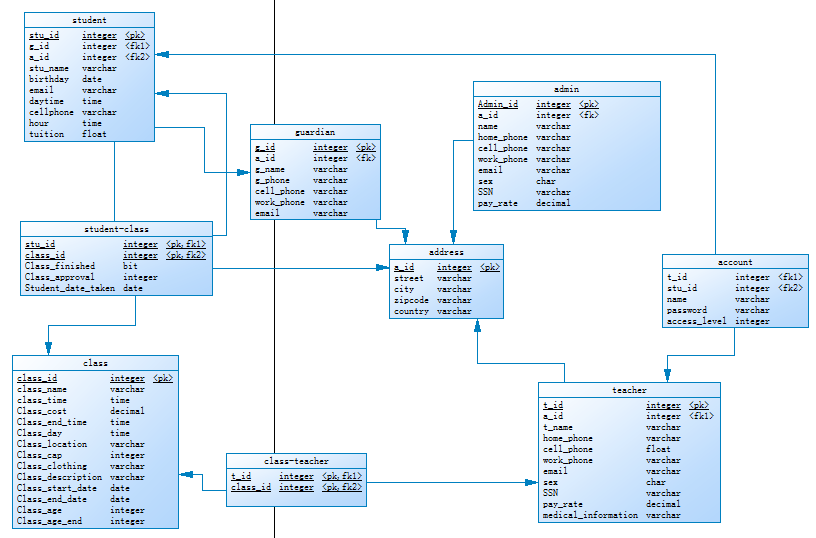
\includegraphics[scale=0.8]{pics/database.png}\\


\subsection{Data Flow Description}
Each table has different purposes for example teacher's table is for storing information of teachers and student's table's is for storing information of student. Different tables are evoked by different functionalities for instance the function of search for students' information will use student and guardians and address tables at same time, and for assign teacher to classes it will use teacher and class and class-teacher table at same time


\section{GUI}
[DW]
\subsection{Technologies  Used}
We mainly use PyQt and Qt Designer for our GUI development.

\subsection{Component  Overview}
There are several components in our GUI design and can be divided into four parts authentication pages, admin pages, teacher pages and student pages.

\subsection{Phase Overview}
\subsubsection{Initial Creation}
We first created login and permission-level pages which is for authentication purposes. Then, we made two landing pages, one is for admins and another is for teachers. Those landing pages contain several sub-pages which corresponding to certain group of functionalities.
\subsubsection{Later Creation}
We are going to add a web interface for student in spring 3.5.\\
(updated in spring 3.5)\\
 
\subsubsection{authentication pages}
It consists of a login page and a permission-level page which to authenticate user and lead them to corresponding landing page.\\
\includegraphics[scale=0.7]{pics/login_page.png}
\subsubsection{admin landing pages} 
It consists of a admin landing page and several sub-pages where admin can perform certain functionalities.\\
\includegraphics[scale=0.7]{pics/admin_landing.png}

\subsubsection{teacher landing pages} 
It consists of a teacher landing page and several sub-pages where teacher can perform certain functionalities.\\
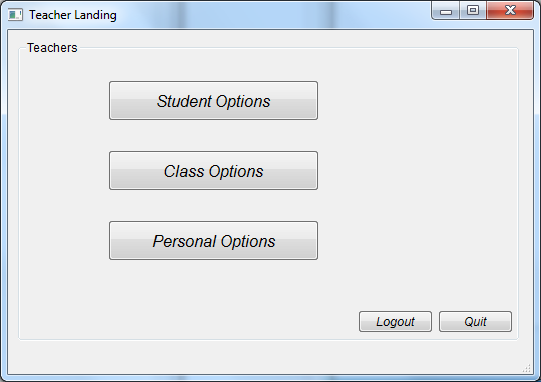
\includegraphics[scale=0.7]{pics/teacher_landing.png}

\subsubsection{student pages}
Need to update in spring 3.5

\subsection{Architecture Diagram}
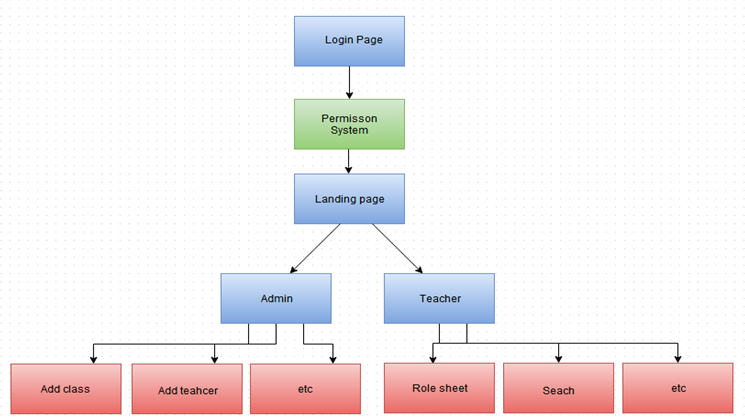
\includegraphics[scale=0.5]{pics/gui.png}\\

\subsection{Data Flow Description}
 Users can log into system through the login page and if username and password are correct then it leads user to permission system which currently is a dialogue box otherwise users get rejected from system. From permission system, user either can be leaded to admin's landing page or teacher's landing page. Then if user is admin they can search employees’ information, add class, add teacher, assign teacher to class, sets clothing requirement for specific class. If users are teachers, they can search students’ information, assign students to class, print the role sheet of the class she is teaching.
In spring 3.5, we also going to add a student web interface and they can use that to register classes and check class schedule. 

\subsection{Design Details}
\subsubsection{Role Sheet Page}
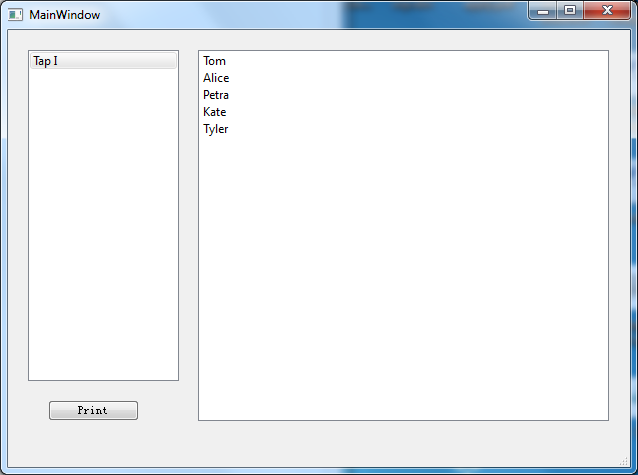
\includegraphics[scale=0.5]{pics/role.png}\\
This window provides a list of classes the teacher, who logs in to system, is currently teaching on the left list view. User can select specific class and it will populate a list of name of student those are in this class\\
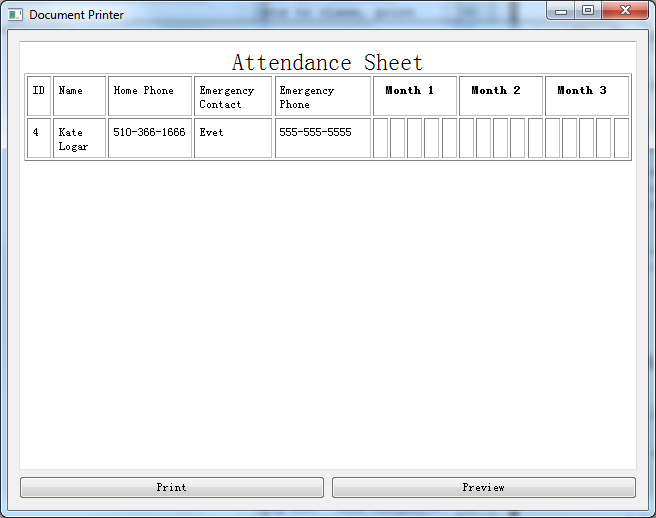
\includegraphics[scale=0.5]{pics/print.png}\\
By clicking print button, it will pop up a window which has the student's names in a text list and user can directly modify names in text list. In later spring, we are going to add some format for the list and make it looks better. User also can import external txt or xml file by clicking open button. Before print use can use preview to generate a pdf with list names of student on it and to see whether it is the list user wants to use. By clicking print button, use can print the actual list.

\subsubsection{Update Form Page}
\includegraphics[scale=0.5]{pics/Update Teacher.png}\\

\subsubsection{Add Information Page}
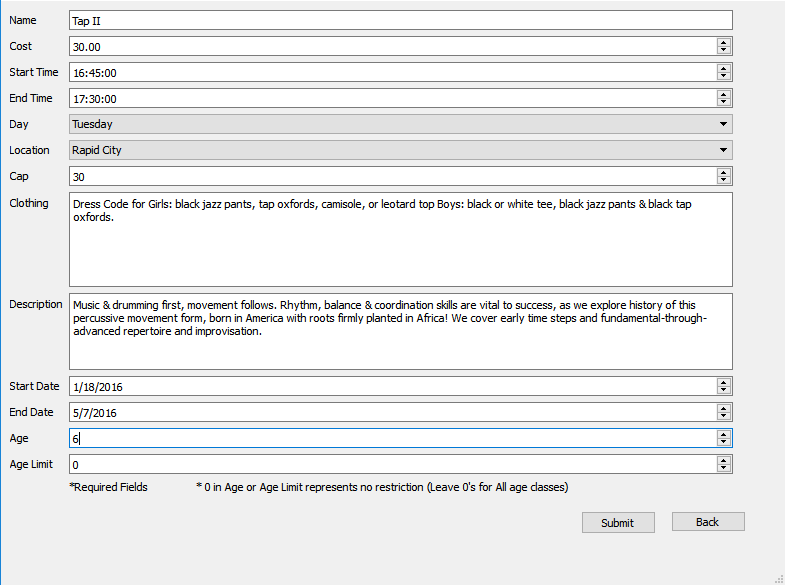
\includegraphics[scale=0.5]{pics/Add_class.png}\\
In the system there is a  multitude of different information that could be added this includes classes, teachers, and students. This is normally done in the system through the use of various forms for data entry.

The forms vary depending on the needs of the entry and will check required field when the submit button is clicked. A dialogue box will pop up asking the user to read over and finalize their entry to the database. The form then closes and the user is returns to the main page for their level.

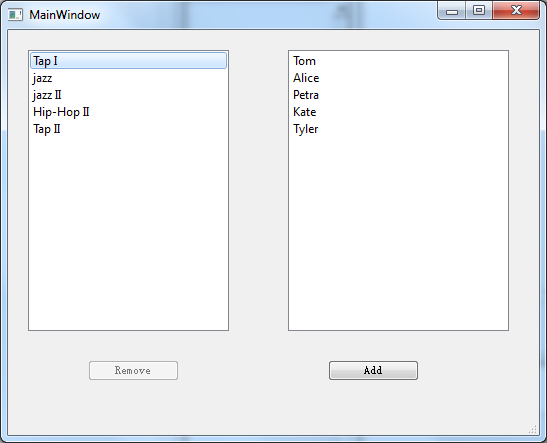
\includegraphics[scale=0.5]{pics/assin_stu.png}\\
This window provides a list of classes which studio are currently running on the left list view. By clicking certain class, it will populate a list of student's names who are in the class for the class on right list view. User can choose specific student and click remove button in order to remove student from class.
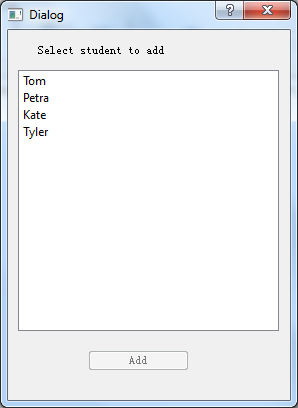
\includegraphics[scale=0.5]{pics/assin_stu_2.png}\\
clicking add button which pops up a dialog containing a list of student's names who are rejected or pending then click add button to add student.

\subsubsection{Search Page}
\includegraphics[scale=0.5]{pics/search.png}\\
This window provides the ability for searching information students and employees. User can search full or partial name by check or uncheck exact box, and it will populate brief information on the table view.
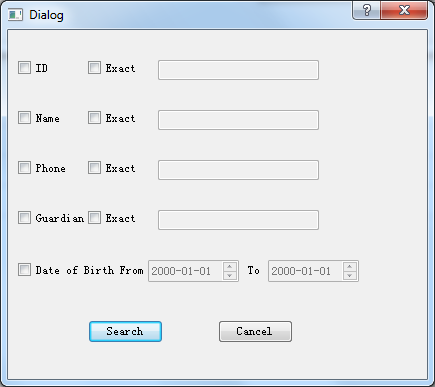
\includegraphics[scale=0.5]{pics/adv_search.png}\\
User can do advanced search by clicking advanced search button. It will let user to choose what kinds of attributes the user wants to use and do the and operation search.\\
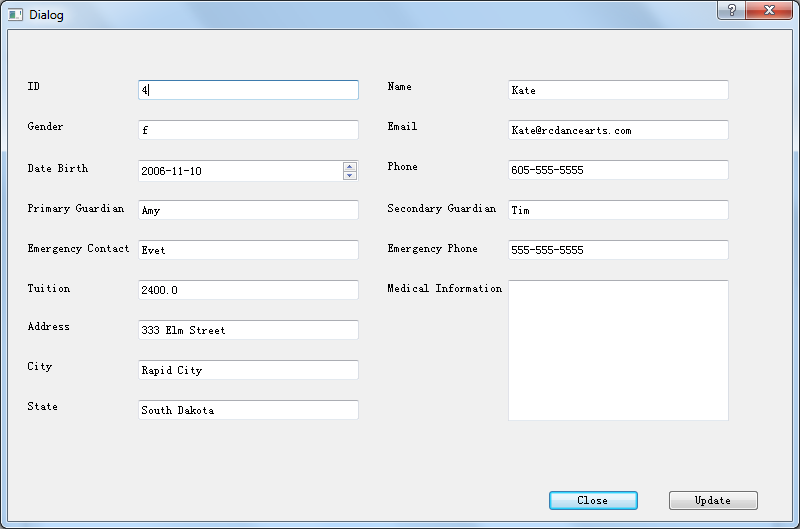
\includegraphics[scale=0.5]{pics/detail.png}\\
User can look into details of each one in the list and click detail button, it will pop up a window that shows detailed information. User also can directly modify information appears in text fields and click submit button to submit new information to database.
\subsubsection{Assign Teacher}
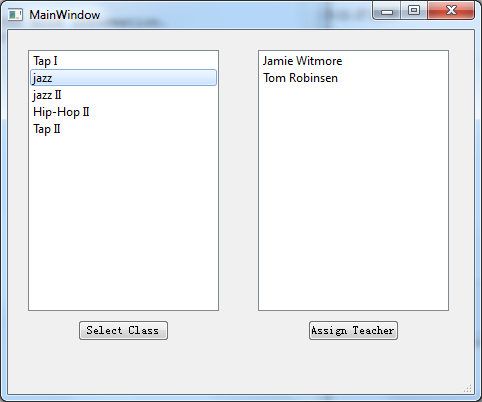
\includegraphics[scale=0.5]{pics/assign_teacher.png}\\
The assign teacher page is how a user will assign a selected teacher to a class. This is done through a window that pops up with two fields. The user will then select a class from the list of classes and a list of available teachers will appear in the right field. The user then selects a teacher and clicks yes on the confirmation message. The system then submits the SQL query to the system with the selected teacher and class. 

If the user selects a classes that is already assigned then the GUI will pop up a message telling the user who is currently assigned to teach the class. The user can then select if they want to change the teacher assigned. If the user selects yes then the right field will populate with a list of other available teachers, retrieved using a query to the database.

  %% All tracks
% !TEX root = SystemTemplate.tex

\chapter{System  and Unit Testing}

This section describes the approach taken with regard to system and GUI testing within the system. 

\section{Overview}
The testing for this project will be done using a GUI test approach through manual and unit test usually done through provided frameworks provided inside either Visual Studio or Xcode and manual checks. Also user test will need to be conducted on the user interface since code based unit test can not be written for certain parts of the user interface, such as navigation flow. The test will be small pieces of code meant to test small sections of code for success or points of failure. The overall goal will be to get as much code tested as possible.

GUI flow and GUI interaction will start as mostly manual testing and if possible automate as much as possible of the GUI testing as possible. [MB] 

\section{Dependencies}
Currently the project contains a few known dependencies in a testing environment. The first is in the PyQt4 Python library which if changed could cause issues within the system GUI and functionality test written for it. However this seems unlikely since the main focus of PyQt updates is now focused on PyQt5. Second is the project dependence on MySQL relational database. This dependency should also be negligible since any update to MySQL are normally done with continuing compatibly with existing software in mind. A third dependency is the RC Dance Arts web page interfacing with the student interface while should not be an issue due to the way the website is constructed since the website is mostly just html. [MB]

\bf (UPDATES WILL NEED TO BE MADE IN LATER SPRINTS AS TESTING FRAMEWORK GROWS PAST MANUAL TESTING) 


\section{Test Setup and Execution}
Test cases for this project were develop by the team to test specific functions and code sections and are therefore developed by the coder to test sections of the code. This can range from a print to test loops or function access to produce a full data entry or a response to test database connects and data modifications.
Depending on the type of test needed the development can take many forms. Such as specific script file test, in which case the test will execute every time the script is run until the test is removed from the code of the script. This form of test is usually used by the team to test loop or other condition statement functionality or any other one off type of code test.
Second is GUI test, user interface test will be conducted in two ways. Buttons and pathways will be manually tested, this means running the program and clicking the buttons to make sure that the window function properly. Second is the GUI's ability to connect and interact with the database in the correct manner. This is done through a combination of manual and script or query test. 


\bf(ADD EXTERIOR SYSTEM, STUDENT INTERFACE, and SYSTEM INTEGRATION TEST AS WRITTEN)
\bf(UPDATE UNIT TEST FRAMEWORK AS PROJECT PROGRESSES PAST MANUAL TESTING)
\bf(CREATE RECORD OF TEST ON STUDENT INTERFACE AND PAYROLL DURING SEMESTER 2) 
\bf(NOTE TO SELF COVER MANUAL TEST LOG BETTER IN SEMESTER 2)
  %% All tracks
% !TEX root = SystemTemplate.tex
\chapter{Development Environment}
The basic purpose for this section is to give a developer all of the necessary 
information to setup their development environment to run, test, and/or develop. 


\section{Development IDE and Tools}
Describe which IDE and provide links to installs and/or reference material. 

\section{Source  Control}
Which source control system is/was used?  How was it setup?  How does a developer 
connect to it? 

\section{Dependencies}
Describe all dependencies associated with developing the system. 

\section{Build  Environment}
How are the packages built?  Are there build scripts? 

\section{Development Machine Setup}
If warranted, provide a list of steps and details associated with setting up a 
machine for use by a developer. 

 %% All tracks
% !TEX encoding = UTF-8 Unicode
% !TEX root = DesignDocument.tex

\chapter{Release -- Setup -- Deployment}
This section contains a list of the deployment dependencies, deployment instruction for future iteration development, development setup instructions, and a brief description of the concept and future versions and development of the DanceSoft product.  


\section{Deployment Information and Dependencies}
The DanceSoft project created by this team is meant to be a proof of concept for the creation of a administrative software for the Academy of Dance Arts. Since this is a first iteration of the software, the system is not meant to be deployed for industrial use at the Academy. The project contains several install dependencies since a actually installer was not developed for this project.\\
In order to run this iteration of the DanceSoft software the user will need to install several separate components, these include:

\begin{enumerate}
\item A valid instillation of Python 3 which can be acquired from \url{https://www.python.org/downloads/}
\item The PyQt 4 libraries and the PyQt designer suite acquired from url{https://www.riverbankcomputing.com/software/pyqt/download}. The product will not work with PyQt 5 without modification due to the incompatibilities between PyQt 4 \& 5
\item A MySQL database that can be used to store data, and possibly a database management software like MySQL Workbench for direct data manipulation and continued development. You can download MySQL free of charge from \url{http://dev.mysql.com/downloads/} and MySQL workbench can be found at \url{http://dev.mysql.com/downloads/workbench}. However any MySQL database manipulation software should work with the project, so the user can use their preferred software.
\end{enumerate}

Once these main three software packages or libraries are installed the user should be able to open all the Python scripts for development or run the "login.py" script to run the software. Other Dependencies for this project include:

\begin{enumerate}
\item The database connection - If the software can not connect to the database either over a network or a local machine, the product will be rendered useless on account of the log in page and most to all pages relying on the database to function correctly.
\item The PyQt 4 libraries - Like with most programming languages and libraries if the standard functions are modified it can break or alter the software functionality. However this should not be a problem when deploying the system due to the main work being done on PyQt 5.
\item PyQt installation - During Deployment if the PyQt libraries are installed incorrectly then the system will fail to deploy/run effectively.
\item MySQL
\item Python 3
\end{enumerate}



\section{Setup Information}
Setup for further development of the DanceSoft has several steps and pieces as no installer was developed within the time frame of this iteration. The following is a general overview of the steps to step up for development of the system.\\

Steps for running the software:\\

\begin{enumerate}
\item Install Python 3
\item Install PyQt 4
\item Install MySQL
\item Download the DanceSoft python scripts
\item Run the login.py script
\end{enumerate}

\subsection{Installing Python 3}
The first major component of the system is the main programming language for this version, Python. Python has two main versions at the time of writing this document, these are Python 2.7 and Python 3.4, the Dancesoft project was developed using python 3.4 and therefore will not work on Python 2.7.
To install Python 3 go to \url{https://www.python.org/downloads/} from this site a developer can download several version installers for Windows, Mac OS X and Linux/UNIX. Once the installer has been run a developer can confirm success by running the Python 3 command from the command line.

\subsection{Installing PyQt 4 and Designer toolkit }

A developer can install the PyQt 4 library from \url{https://www.riverbankcomputing.com/software/pyqt/download}. The PyQt 4 library can also be copied from the DanceSoft git repo located at \url{https://github.com/SDSMT-CSC464-F15/dancesoft}.

The riverbank website contains installers for the PyQt library that include all needed components for the system. On Mac or Linux user can download the snips or source code from the website, or use one of the many tutorials online if needed. The team recommends just copying the files from the repo and placing the PyQt folder in the site-packages sub-folder of the Python 3 folder. 

\subsection{Installing MySQL}
The database component used by the team was MySQL, this software can be download and installed free of charge from \url{http://dev.mysql.com/downloads/}. Further manipulation software such as MySQL Workbench, or Navicat can be installed to help with development. Several pieces of  software can also be found on the MySQL website, however any MySQL development software can be used. It is up to future developers to find the software that fits their needs the best.

\subsection{Running Project}
Once all the necessary components have been downloaded and installed a developer can write/run the Python and PyQt scripts for the project. To start the current system the user must run the "login" script to pull up the log in window and begin using the software. 

At the time of project submittion the project contained an admin log in using the user name: jwitmore and the password: rcdance. This account was used both for testing and client demo purposes during the initial program development.

\section{System Version Information}
Past version of this system have been presented to the client as senior design projects, however due to reasons unknown by this team the projects were abandoned by the client. Therefore the previous versions have no effect or input on this teams proof of concept for the DanceSoft system. 

The system is in a pre-industrial version noted in this document as version 1.x.x this iteration of the DanceSoft project is a proof of concept presented to the client Jeff McGough. The idea of this first iteration is to show that a true in use launch of this software is possible. Whether this is through a follow up senior design team that will use this teams iteration as a blueprint, Dr. Jeff McGough continuing development himself, or finishing the project through a contractor, or industrially mentored senior design team.

This version shows execution of the main functions laid out in the initial requirements. These functions provide an ideas for a minimum viable software. The first version of the software was meant to have a full interface and a student web portal for student registration, billing, and information management. However due to time constraints, DanceSoft team issues, and to many other academic commitments from the two members of the DanceSoft team, the client converted the projects goals from a industrial launched product to a proof of concept for future iteration and versions. 

Future versions of the software however the client may choose to create them will most likely include more refined functionality, the addition of the student web portal if possible, more database concurrency, and security. Even though the current version is a proof of concept as described in the DanceSoft software contract; It is the belief of this team that the final version of this software is possible through future iterations, and versions.


\section{Future Work}
The following is the remaining work that needs to be done on this project should this iteration be directly continued. If the project proceeds using different tools or to a contract job, this section can be ignored.

\begin{enumerate}
\item The project and database are currently not secure, security will need to be implemented in the system.
\item The student web portal
\item The connections in the local GUI to the student web portal
\item The billing and payroll functions are currently very rough, and will most likely be redone in the future.
\item Importing and Exporting data to the database
\item Database backups
\item A different class hours rate for each teacher since all employees are not paid the same for class time.
\item Refunds and an old version of the Add/Drop students where left in at the request of the client, but overall serves no purpose within the system.
\item Fees are listed in the system however they do not currently do anything else within the system
\item Family billing and setting discounts where not implemented in this version of the system.
\end{enumerate}


  %% Normally not research track
% !TEX root = DesignDocument.tex


\chapter{User Documentation}

\section{User Guide}

The following is the user guide for the DanceSoft project:

\subsection{Entering the Software}
Login page:\\
When the user first logs into the system the user is prompted with a log in window where they can enter their user name or pass word for the system. If the user enters the wrong password then the system pops up a dialog and tells the user to reenter there password. The default user name for a new user is the name used to enter the system. So if I enter a new teacher named Marcus Berger then the default user name is Marcus Berger. The default password is rcdance, both the user name and password can be changed using the change functions in the personal section of the teacher landing page.\\

\begin{figure}
  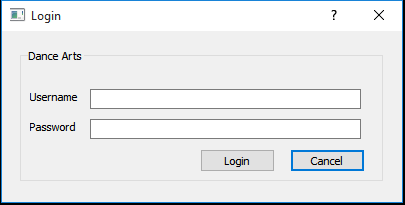
\includegraphics[width=\linewidth]{pics/userGuide/login.png}
  \caption{Log in page}
  \label{fig:User doc: log in}
\end{figure}

Landing Selection:\\
After the user logs in they can select which of the two landing pages, Admin or Teacher that they want to go to. If the user does not have admin permissions the user will be blocked from going to the Admin Landing page.\\

\subsection{Admin Landing}
Once an admin has logged in they can select the admin landing page to be taken to a variety of functions listed below. 
In the main page the user has four options for type of functions to choose from employee, student, class, and billing.\\

\begin{figure}
  \includegraphics[width=\linewidth]{pics/userGuide/admin_landing.png}
  \caption{Admin Main Page}
  \label{fig:User doc: Admin Landing}
\end{figure}

\subsubsection{Manage Employees} 
When the user clicks on manage employee they are given a set of buttons that they can choose from.\\

Search Teacher:\\
When the user selects search teacher, the system will bring up a window that displays the teachers in the system. The user can then type a teacher's name into the search bar and the field will display the teachers that names contain the entered value. If the user is looking for an exact match then they can check the "exact check box. After the user conducts a search, they can click the refresh button to bring back the full list of teachers in the database.

By clicking the advanced search button the user can further refine the search value, the advanced search dialog is accessed by clicking the advanced search button. Advanced search allows the user to to search for teachers by id, name, phone numbers, or date of birth.

One the users desired teacher is found the user can click on the name in the main window and select a details button to view all the information for that teacher.  In the details window the user is able to change the information for an entry and submit the updates to the system.\\

\begin{figure}
  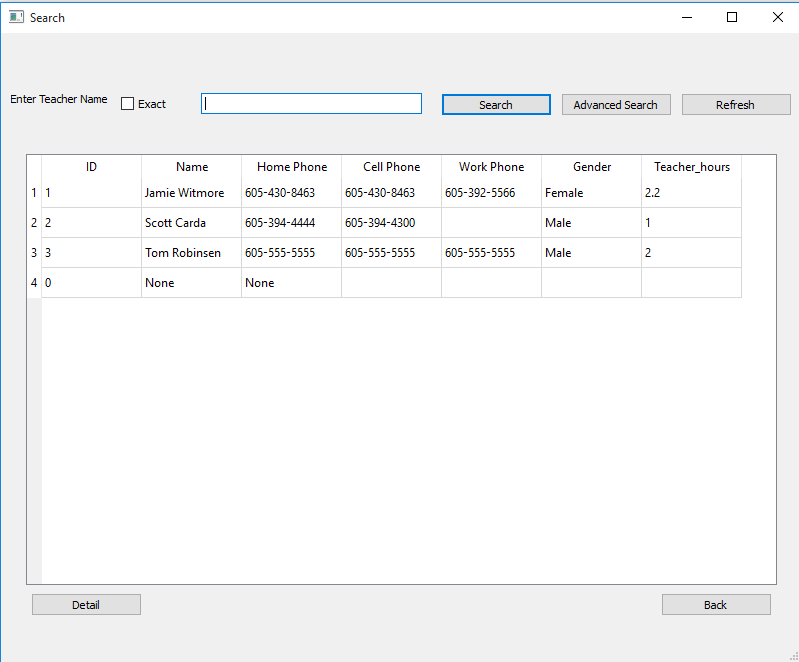
\includegraphics[width=\linewidth]{pics/userGuide/teacherSearch.png}
  \caption{Teacher Search Window}
  \label{fig:User doc: Teacher Search}
\end{figure}

Show Admin List:\\
On the main admin page the user can select the admin list button. This will display a text list of admins for the system. The window contains a search bar to refine the list if the user is looking for a specific entry. The page contains a details button which will allow the user to view the full details of the entry. The add button allows the user to select a teacher in the system and give them admin permissions.  The remove button allows the user to remove admin permissions from the system, this however does not remove the teacher from the system.\\

Update Teacher Information:\\
The update teacher button on the admin employee page, allows the user to select a teacher in the system and one selected a form will be populated. The user can then change any of the fields and submit the updates to the systems database.\\ 

\begin{figure}
  \includegraphics[width=\linewidth]{pics/userGuide/updateTeacher.png}
  \caption{Update Teacher Form}
  \label{fig:User doc: Teacher Update}
\end{figure}

Enter Teacher Hours:\\
Another button on the admin landing page is "Enter Teacher Hours". The user is able to select a teacher and a dialog pops up. The user is then able to view the selected teachers hours in each pay rate and change them if the user so chooses. The gross wage is then calculated and displayed to the user.\\

\begin{figure}
  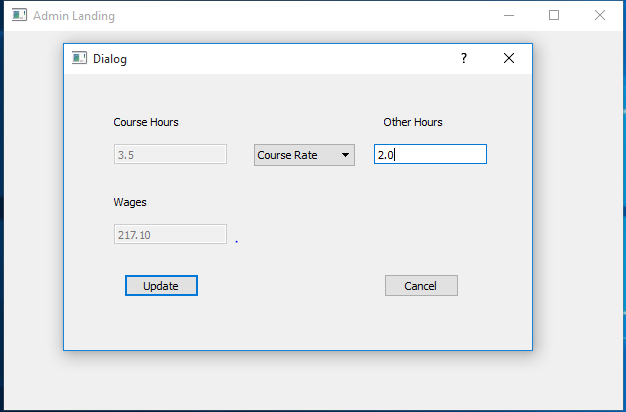
\includegraphics[width=\linewidth]{pics/userGuide/hours.png}
  \caption{The Admin Hours Page}
  \label{fig:User doc: Enter Hours}
\end{figure} 

Assign Teacher to Class:\\
This button bring up the assign teacher window. From here the user is able to select a class name, if the class is currently assigned to a teacher a dialog box will pop up asking the user if they would like to reassign the class to a different teacher. If the user selects yes or if the selected class is currently not assign to a teacher a list of teachers available at the class time will pop up and the user can select a teacher to assign to the class.\\

\begin{figure}
  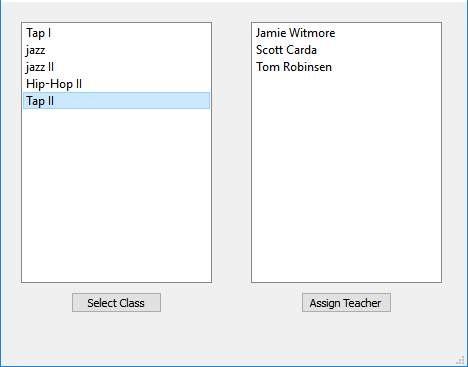
\includegraphics[width=\linewidth]{pics/userGuide/assignClass.png}
  \caption{Assign Class Window}
  \label{fig:User doc: Assign Class}
\end{figure} 

Teaching History:\\
The user is able to select a teacher and press the history button, this brings up a list of all the classes that teacher has taught, excluding the current semesters classes.\\

\begin{figure}
  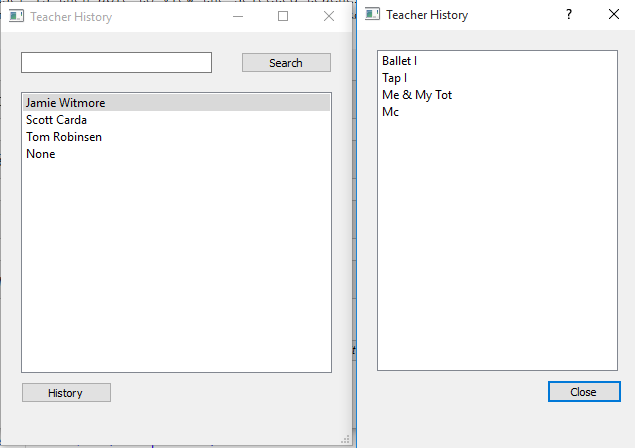
\includegraphics[width=\linewidth]{pics/userGuide/history.png}
  \caption{Teacher History}
  \label{fig:User doc: Teacher History}
\end{figure} 

Enter New Teacher:\\
This button ups a form where the user can enter the fields for a new teacher. Once all the required fields are filled out the user can submit the teacher to the system. The required fields are name, date of birth, home phone, address fields, gender, and SSN. When the submit button is clicked, the user will be able to review the entry before submitting it to the system.\\

Remove Teacher\\
The user is able to select the name of a teacher and remove the selected teacher from the system. This removal is complete, this means that if the user removes a teacher it will completely remove all the data from the system connected to that teacher. This includes classes, teacher data, and hours.\\

\subsubsection{Manage Classes}

View Classes\\
This button allows the user to search classes like in the teacher search explained above. The general functionality is the same, the user is able to search by class name and refresh the view window after a search. The user can check the exact button if they wish to look only for what they entered. The Advanced search button allows the user to search for classes based on id, name location and time. Once the desired class is found the user can select a class and press the details button in order to view the full details for a course. Within this details page the user can modify the information and send updates to the system.\\


\begin{figure}
  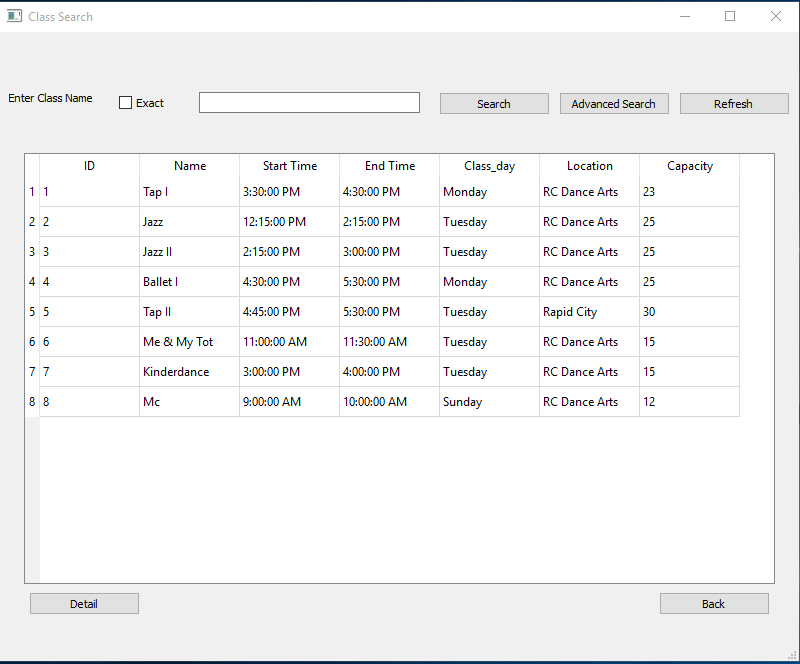
\includegraphics[width=\linewidth]{pics/userGuide/classSearch.png}
  \caption{Class Search Window}
  \label{fig:User doc: Class Search}
\end{figure}

Add a Class:\\
A form will pop up where the user can enter in all the information needed to add a class. Once the user has entered in all the information and clicked submit a dialog will pop up where the user can check and confirm the submission. Selecting "Add New Location" in the location drop down will pop up a dialog box which will allow the user to enter in a new location for the class, the user can also select a location that already exist in the system.\\

Remove Class:\\
The user is able to select the name of a class and remove the selected class from the system. This removal is complete, this means that if the user removes a class it will completely remove all the data from the system connected to that class. This includes class data, removal from schedules, removal from any billing calculations, and any pending registrations\\

Set Semester:\\
Allows the user to select the current semester in the system or add a new semester.

\begin{figure}
  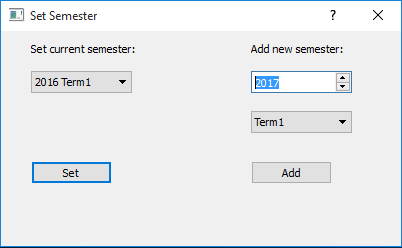
\includegraphics[width=\linewidth]{pics/userGuide/setSemester.png}
  \caption{Set Semester Window}
  \label{fig:User doc: Set Semester}
\end{figure}

\subsubsection{Manage Students}

Search Students:\\

When the user selects search student, the system will bring up a window that displays the students in the system. The user can then type a student's name into the search bar and the field will display the students that names contain the entered value. If the user is looking for an exact match then they can check the "exact check box. After the user conducts a search, they can click the refresh button to bring back the full list of students in the database.

By clicking the advanced search button the user can further refine the search value, the advanced search dialog is accessed by clicking the advanced search button. Advanced search allows the user to to search for students by id, name, phone, guardian or date of birth.

One the users desired student is found the user can click on the name in the main window and click a details button to view all the information for that student.  In the details window the user is able to change the information for an entry and submit the updates to the system.\\

\begin{figure}
  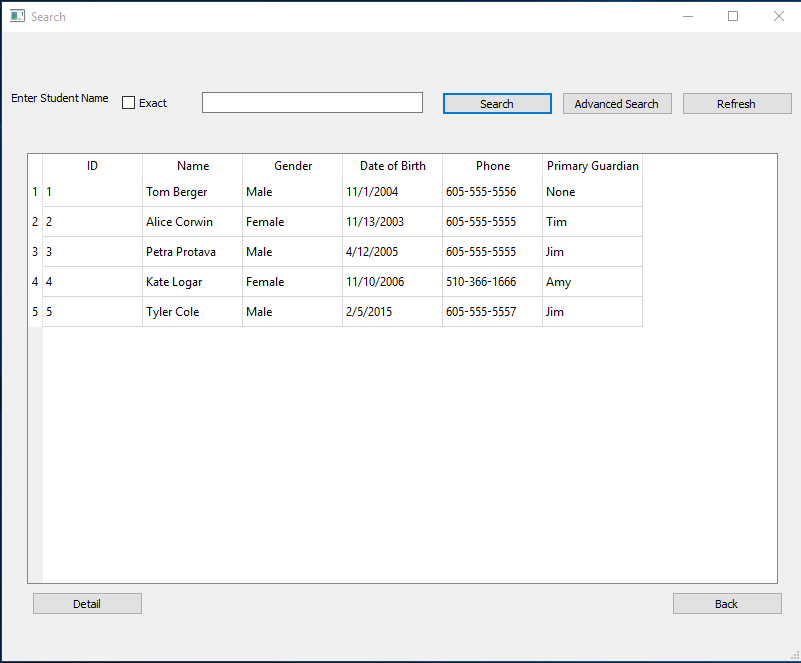
\includegraphics[width=\linewidth]{pics/userGuide/searchStudents.png}
  \caption{Student Search Window}
  \label{fig:User doc: Student Search}
\end{figure}


Student Credits:\\
This button will pull up a window where the user can select a students name and their credit amount within the system will be displayed. The user can then update the credit amount for that student. The credits are not factored into any student billing calculations. This is in accordance with the Academy of Dances Arts refund and credit policy as the credits and refund distribution is up to the users of the system. One the credits have been used the user must reset the reset the students credits to zero.\\

\begin{figure}
  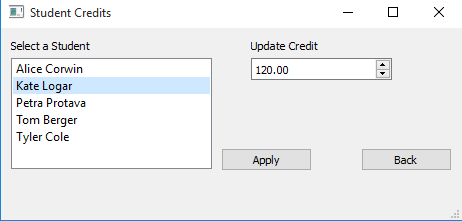
\includegraphics[width=\linewidth]{pics/userGuide/credits.png}
  \caption{Student Credit Window}
  \label{fig:User doc: Student Credits}
\end{figure}

Add/Remove Student:\\
This button brings up a window that allows the user to select a class. Once a class is selected the students currently registered will appear along with their class approval status. User can then select a student name and either click the add button to set the approval to one meaning the student is approved to take the class. A user can also remove the student which sets the approval to negative one meaning rejected. An approval of zero means the students registration is pending.

This function was created for the student interface links, however this set of functions were dropped so this function was left in at the request of the project's initial client Dr. Jeff McGough, so a future iteration of the project could see it. However in the projects current state this window serves no real overall purpose and should not be used by any users of the software. Anyone wishing to do student registration should do so through the student registration function explained below.\\


\begin{figure}
  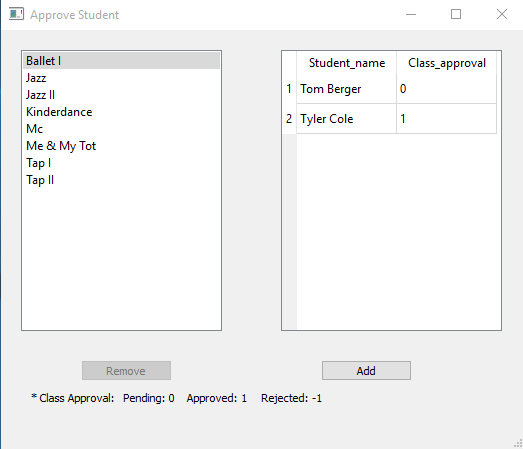
\includegraphics[width=\linewidth]{pics/userGuide/Addstu.png}
  \caption{First Student Registration}
  \label{fig:User doc: First Student Registration}
\end{figure}

Registration:\\
The user is able search for a preexisting and select a student. The user can then click the "Update" button to bring up the details of that student, the user can then change and update the student's information in the system.  Once the updates are made or if there are no information updates the user can click the "list" button and bring up a list of classes the student is currently registered for and the classes the student can register for. Classes can be dropped by selecting the class and clicking the drop button. Classes can be added from the pending class section using the add button.

Back on the student list window instead of clicking the "Update" button, the user can click the "Add" Button and enter in a new students information. If the  new students guardian is not in the system the user can click "Add Primary" to add the student's primary guardian. If the student needs a new secondary guardian the user can click the "Add Secondary" button and add another guardian to the system.  Once all the information for the student has been added the user can click the "Add" button to finalize the student.

\begin{figure}
  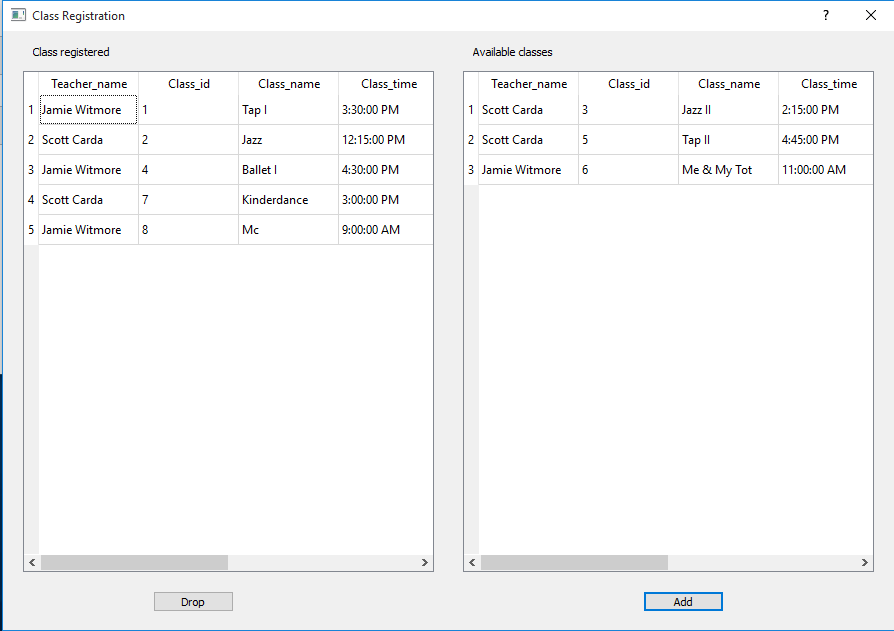
\includegraphics[width=\linewidth]{pics/userGuide/studentReg.png}
  \caption{Current Student Registration Window}
  \label{fig:User doc: Student Registration}
\end{figure}

\begin{figure}
  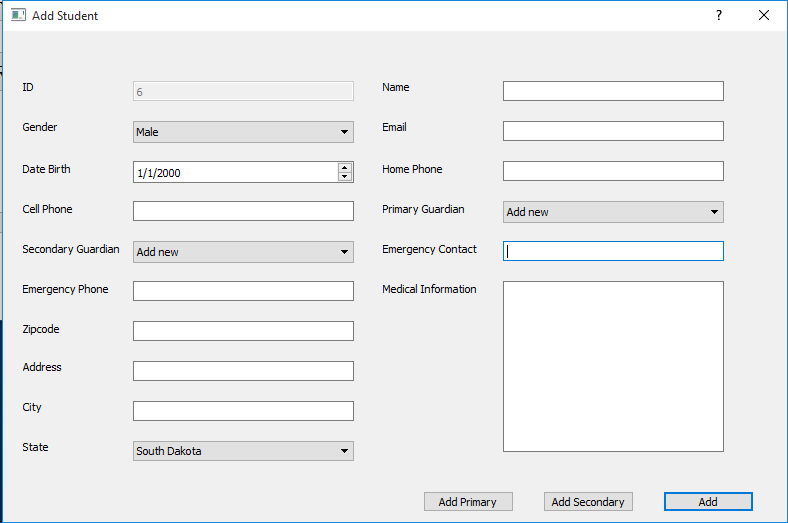
\includegraphics[width=\linewidth]{pics/userGuide/AddStudent.png}
  \caption{Add New Student Window}
  \label{fig:User doc: Add Student}
\end{figure}

Remove Student:\\
The user is able to select the name of a student using a search bar and remove the selected student from the system. This removal is complete, this means that if the user removes a student it will completely remove all the data from the system connected to that student. This includes class data, removal from schedules, removal from any billing calculations, any pending registrations, and if no other students such as sibling are connected to an address or a guardian the address and/or guardians will be removed as well. Any remove functions should be done with caution\\

\subsubsection{Manage Billing}
These functions are the general billing function for this version of the software ane allow the user to handle the base level billing functionality of the DanceSoft project.\\

Enter Partial Payment:\\
The User is able to search for a student and select them. When the user selects a student that is making a payment a window will appear where the user can type in the amount paid by the student. The type of payment is selected from a drop down menu, this value is used in the billing history to display how the student paid. The last combo box allows the user to select the term in which the payment was made. The payment is processed when the user clicks "Confirm."\\

\begin{figure}
  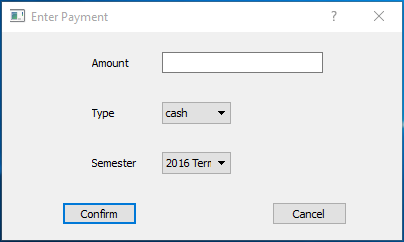
\includegraphics[width=\linewidth]{pics/userGuide/partPay.png}
  \caption{Partial Payment Window} 
  \label{fig:User doc: Partial Payment}
\end{figure}
  
Enter Full Payment:\\
Enter full payment works the same way as partial payment the user is able to search for an select a student, however instead of entering a payment by clicking the button the students owed amount will be set to zero.\\

Enter Teacher Pay Rate:\\
The Enter Teacher Pay Rate button opens up a window where the user can select a teacher. Once a teacher is selected the user can open the pay rate window. From the pay rate window the user can enter a new pay rate for the current teacher and the amount that pay rate is worth. The user can them add the pay rate to the system by clicking the "Add" button. If the user chooses to update the pay rate the user can select the rate they wish to update from the drop down menu and change the value in the box. The update is submitted by clicking the update button. Currently the added pay rates are for that teacher, but the course rate is the same among all teachers. Future versions should add the ability to have different course rates for each teacher.\\\

\begin{figure}
  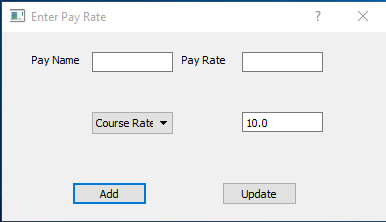
\includegraphics[width=\linewidth]{pics/userGuide/enterPay.png}
  \caption{Enter Pay Rate Window} 
  \label{fig:User doc: Enter Pay Rate}
\end{figure}

Student Balance:\\
The user selects a student and can clicks the "Statement" button. The students statement will produce a name, the current semester, the classes taken that semester, the total money paid, due, and the remaining balance. The user can print out the statement as well if needed.\\

\begin{figure}
  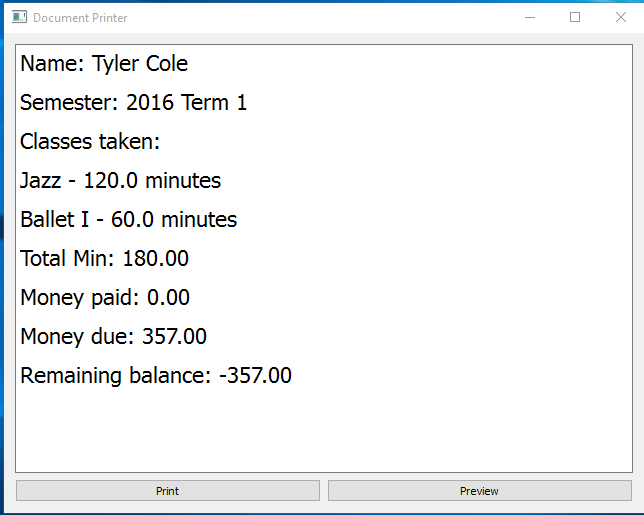
\includegraphics[width=\linewidth]{pics/userGuide/stuBalence.png}
  \caption{Student Balance Window} 
  \label{fig:User doc: Student Balance}
\end{figure}

Billing History:\\
When the user clicks the "Billing History" button, a window appears where the users can search for and select a student. Once a student is selected the user can click the statement button and produce the payment list for a student. The payment list contains the name of the student, the term the payment was made for, the amount paid, and the date the payment was made. The user can print the statement if they want to using the print button.  

\begin{figure}
  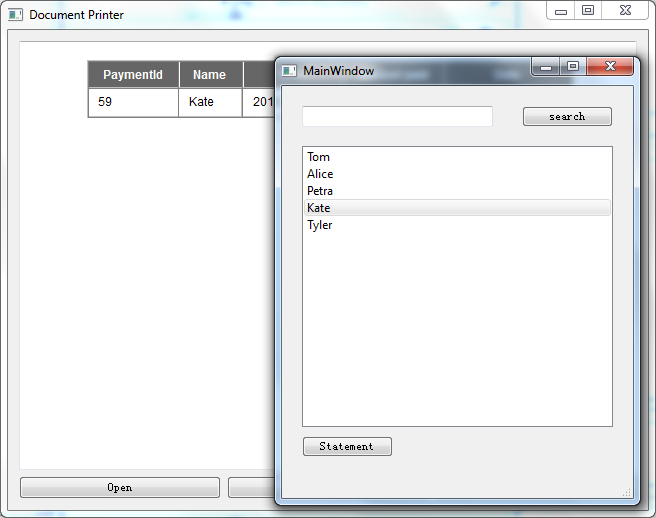
\includegraphics[width=\linewidth]{pics/userGuide/billHistory.png}
  \caption{Student Billing History} 
  \label{fig:User doc: Billing History}
\end{figure}

Tuition Rates and Fees:\\
The user is able to view all the tuition rates in the system and update them if need be, by changing the values of in the boxes. The user can also add and remove tuition rates as well. In the fee window the user can add a fee update a fee in the system and remove a fee it they so choose. However as of this version of the project none of the fees are factored in to any of the calculations. In future versions the project should be able to connect the fees to billing calculations. The tuition rates are based on the amount of minutes and they in turn determine the amount a student owes. If these are changed or remove it could mess with the way the system does billing for the Academy. Handle with caution. In future iterations teams should be able to better connect these systems.

\begin{figure}
  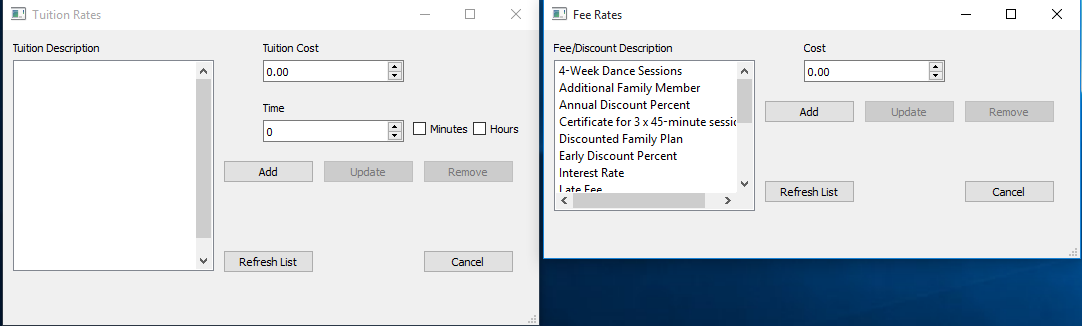
\includegraphics[width=\linewidth]{pics/userGuide/tuitAndFees.png}
  \caption{Tuition and Fees} 
  \label{fig:User doc: Tuition and Fees}
\end{figure}


\subsection{Teacher Landing}

\subsubsection{Student Options}

Search Students:\\
When the user selects search student, the system will bring up a window that displays the students in the system. The user can then type a student's name into the search bar and the field will display the students that names contain the entered value. If the user is looking for an exact match then they can check the "exact check box. After the user conducts a search, they can click the refresh button to bring back the full list of students in the database.

By clicking the advanced search button the user can further refine the search value, the advanced search dialog is accessed by clicking the advanced search button. Advanced search allows the user to to search for students by id, name, phone, guardian or date of birth.

One the users desired student is found the user can click on the name in the main window and click a details button to view all the information for that student.  In the details window the user is able to change the information for an entry and submit the updates to the system.\\

\begin{figure}
  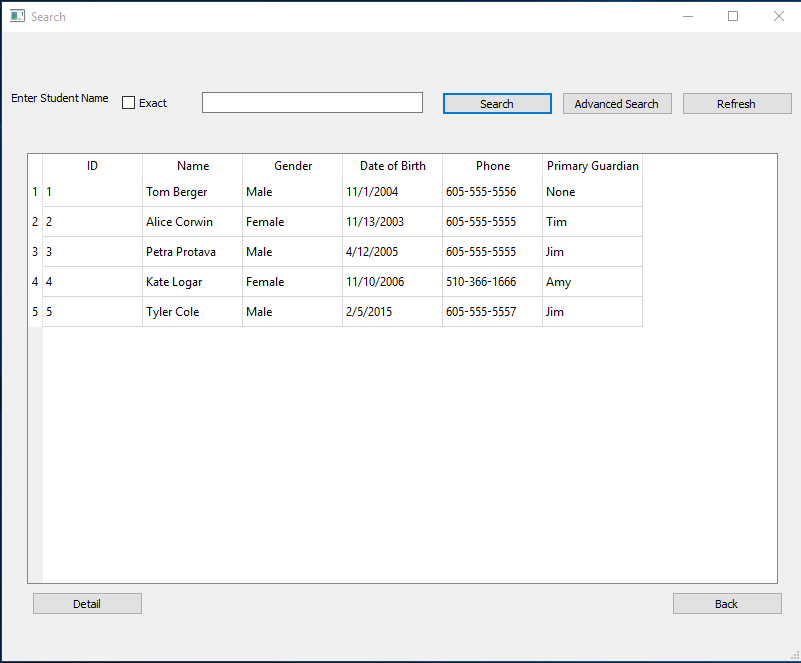
\includegraphics[width=\linewidth]{pics/userGuide/searchStudents.png}
  \caption{Student Search Window}
  \label{fig:User doc: Student Search}
\end{figure}

Add to Class:\\
This button brings up a window that allows the user to select a class. Once a class is selected the students currently registered will appear along with their class approval status. User can then select a student name and either click the add button to set the approval to one meaning the student is approved to take the class. A user can also remove the student which sets the approval to negative one meaning rejected. An approval of zero means the students registration is pending.

This function was created for the student interface links, however this set of functions were dropped so this function was left in at the request of the project's initial client Dr. Jeff McGough, so a future iteration of the project could see it. However in the projects current state this window serves no real overall purpose and should not be used by any users of the software. Anyone wishing to do student registration should do so through the student registration function explained below.\\

Student Schedule:\\
This button allows the user to pull up a window where they can select a student and view there class schedule. The user can also print out their schedule by pressing the print button. The schedule is design to only display the times that the student is in a class.\\

\begin{figure}
  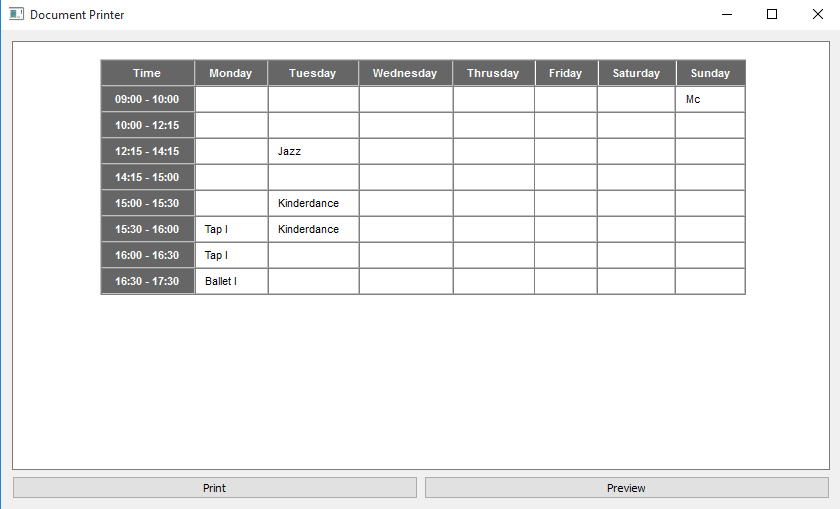
\includegraphics[width=\linewidth]{pics/userGuide/studentSchedule.png}
  \caption{Student Schedule Window}
  \label{fig:User doc: Student Schedule}
\end{figure}


\subsubsection{Class Options}
This section contains the class related function that a teacher may need to manage their day to day activities.

View Classes:\\
This button allows the user to search classes like in the teacher search explained in the admin section. The general functionality is the same, the user is able to search by class name and refresh the view window after a search. The user can check the exact button if they wish to look only for what they entered. The Advanced search button allows the user to search for classes based on id, name location and time. Once the desired class is found the user can select a class and press the details button in order to view the full details for a course. Within this details page the user can modify the information and send updates to the system.\\


Class Schedule:\\
This button allows the user to pull up a window where they can select a teacher and view there teaching schedule. The user can also print out their schedule by pressing the print button. The schedule is design to only display the times that the teacher is teaching a class.\\

\begin{figure}
  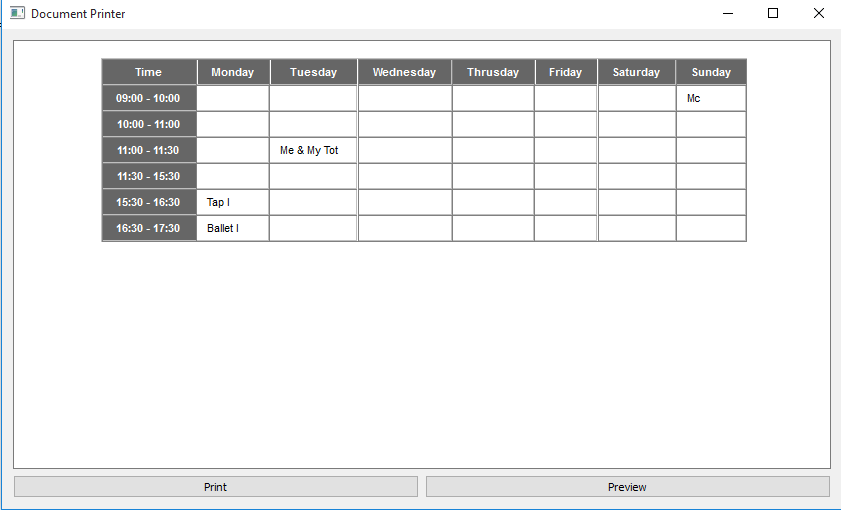
\includegraphics[width=\linewidth]{pics/userGuide/teacherSchedule.png}
  \caption{Teacher Schedule}
  \label{fig:User doc: Teacher Schedule}
\end{figure}


Class Role Sheet:\\
This button creates a window which contains the classes the logged in teacher is currently teaching. The user can click on a class to view the students in the class. If the user wants a formatted role sheet they can click the print button which allows the user to print out a role sheet for the class. The role sheet contains the students name, and emergency contact information, along with a check box for each week in a three month period. This format is accordance with the one a week classes offer at the Academy of Dance Arts.\\

\begin{figure}
  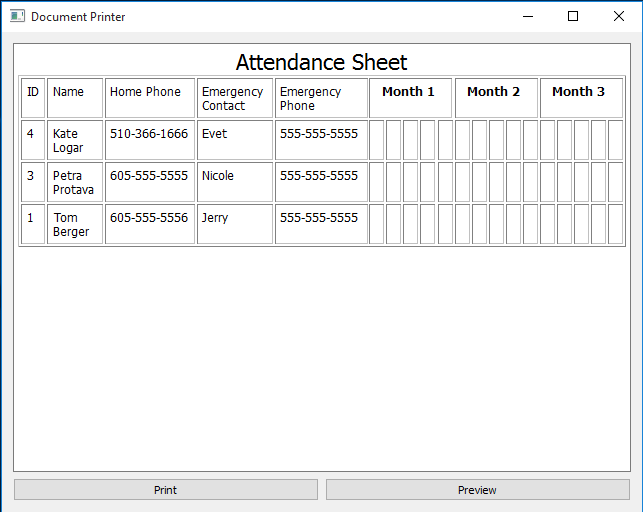
\includegraphics[width=\linewidth]{pics/userGuide/role.png}
  \caption{Class Role Sheet}
  \label{fig:User doc: Class Role Sheet}
\end{figure}

\subsubsection{Personal Options}
This section contains the functions connected to modify information directly connected to the user. These function include change password, change user name, modify personal information, and enter hours.

Change Password\\
When using this function the user is prompted with a dialog box, form this dialog the user will enter their user name, their desired new password, and confirm the new password. The user will be prompted to reenter their password if their user name or password are incorrect.\\

Change Username:\\
When using this function the user is prompted with a dialog box, form this dialog the user will enter their user name, their password, and the desired new user name. The user will be prompted to reenter their user name if their user name or password are incorrect.\\

Modify Personal Information:\\
If the user ever needs to change their personal information they can click this button to bring up a form containing their personal information. In this form the user can change their name, date of birth, phone numbers, address, and other information within the system. Like the other update teacher form in the admin section of the DanceSoft project, if the user leaves any of the required fields open they will be prompted to fill them in. Also if the user changes their address they will be given a dialog box asking if they would like to update their existing address or create a new one within the database. This is done because if two people going to, or working at the Academy live at the same address the teacher can create a new entry so that the other person address does not get effected. However if the teacher is the only one living at the address the system does not want to create dead data within the database, so the user is given an with an ability to change the entry. 

As stated the user should use caution when ever changing address because if a user updates an address that someone else lives at then that person will have incorrect data, also if a teacher is the only person in the database with an address and a new address is added instead of updating then dead data will be created, and in this project iteration a user would need to access the database directly to remove a dead address as address removal is linked to teacher and student removal.

Enter Hours:\\
The user is able to look through the pay rates linked to their account by system admin and log hours for the various pay rates.


\section{Installation Guide}
The following is the steps to install the DanceSoft software on a users machine:

\bf Step 1: \rm
	The first thing a user needs to do is make sure that a valid version of Python 3 can run on their system, if you already have python 3 installed on your machine please skip to step 2.
	The most recent version of Python 3 can be found on \url{https://www.python.org/downloads/} the user can then click on the download link and download a python zip file that is compatible with the operating system being used by the user.
	Follow the instruction on the install, one the install is complete the python files should be located in your local drive unless the user specified a different directory during install. A user has several ways of confirming that python installed correctly on their system. If the user is  with the command prompt they can run the Python 3 command to confirm successful installation. If the user would like to confirm using non-command line, the user can go to the python 3 file on their drive and run the Python.exe file. If a command window appears then the user has successfully installed python and can proceed to step 2.
	
\begin{figure}
  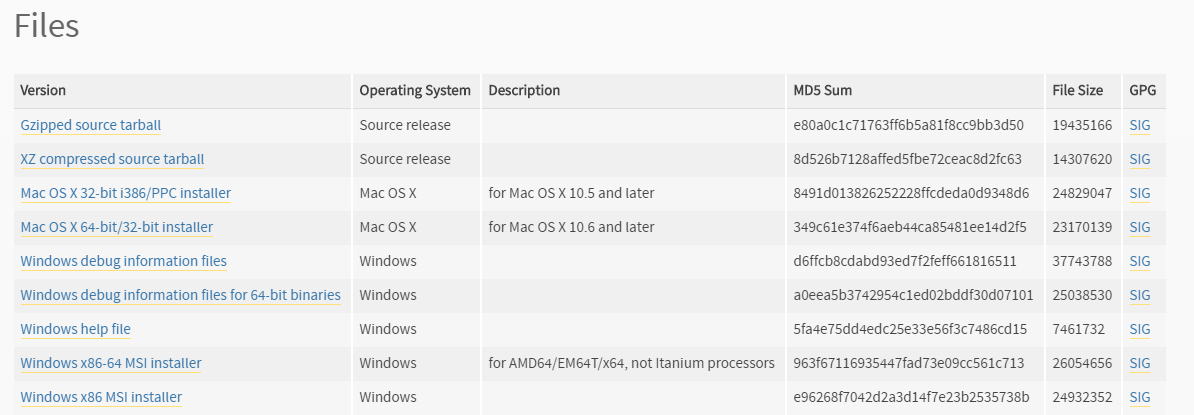
\includegraphics[width=\linewidth]{pics/pythonFiles.png}
  \caption{Python zip files}
  \label{fig:User doc: python files}
\end{figure}

\bf Step 2: \rm
	The next step is to install the PyQt libraries and the designer so the user can run the scripts containing PyQt code. There are several versions of PyQt, the version the DanceSoft team used was PyQt4. PyQt4 can be downloaded from \url{https://www.riverbankcomputing.com/software/pyqt/download}, one there the user can select the zip file that goes with their operating system. The website also provides stable windows installers if the user is running a windows system. If the installer is used the libraries will automatically be stored in the site-packages sub-directory of the python folder and the user should be able to start using PyQt libraries
	If the user is not running windows, they can download and use the brew facility to easily install the need files. If the user runs \bf brew install PyQt --with-python3 \rm from the OS X command line the system should automatically install the needed files.
	 Otherwise the user will need to download the snippets from \url{https://www.riverbankcomputing.com/software/pyqt/download} and install the PyQt libraries in the site-packages folder.
	 
\bf Step 3: \rm
	The last major install a user will need to do before using the software is the MySQL database software necessary to use the SQL components of the DanceSoft project.
	MySQL can be installed by following the download instructions on \url{https://www.mysql.com/downloads/} and downloading the free version of the software. This installer will install all the tools needed to manipulate and use the database directly if necessary.\\
	
The user should now have all the needed tools installed to run the DanceSoft Software.
	 
	


%% \newpage  %%  if needed ...
%\section{Programmer Manual}

 %% All tracks
% !TEX root = SystemTemplate.tex

\chapter{Class Index}
\section{Class List}
Here are the classes, structs, unions and interfaces with brief descriptions\-:\begin{DoxyCompactList}
\item\contentsline{section}{\hyperlink{class_poly}{Poly} }{\pageref{class_poly}}{}
\end{DoxyCompactList}

\chapter{Class Documentation}
\hypertarget{class_poly}{\section{Poly Class Reference}
\label{class_poly}\index{Poly@{Poly}}
}
\subsection*{Public Member Functions}
\begin{DoxyCompactItemize}
\item 
\hyperlink{class_poly_aa3def076b74bed67904976ad4f9fe9b1}{Poly} ()
\item 
\hyperlink{class_poly_a2f8530284140c31c0aa391dd4d0b61be}{$\sim$\-Poly} ()
\item 
int \hyperlink{class_poly_a14a7ad77ce612b0c54f531d307ee4b39}{myfunction} (int)
\end{DoxyCompactItemize}


\subsection{Constructor \& Destructor Documentation}
\hypertarget{class_poly_aa3def076b74bed67904976ad4f9fe9b1}{\index{Poly@{Poly}!Poly@{Poly}}
\index{Poly@{Poly}!Poly@{Poly}}
\subsubsection[{Poly}]{\setlength{\rightskip}{0pt plus 5cm}Poly\-::\-Poly (
\begin{DoxyParamCaption}
{}
\end{DoxyParamCaption}
)}}\label{class_poly_aa3def076b74bed67904976ad4f9fe9b1}
My constructor \hypertarget{class_poly_a2f8530284140c31c0aa391dd4d0b61be}{\index{Poly@{Poly}!$\sim$\-Poly@{$\sim$\-Poly}}
\index{$\sim$\-Poly@{$\sim$\-Poly}!Poly@{Poly}}
\subsubsection[{$\sim$\-Poly}]{\setlength{\rightskip}{0pt plus 5cm}Poly\-::$\sim$\-Poly (
\begin{DoxyParamCaption}
{}
\end{DoxyParamCaption}
)}}\label{class_poly_a2f8530284140c31c0aa391dd4d0b61be}
My destructor 

\subsection{Member Function Documentation}
\hypertarget{class_poly_a14a7ad77ce612b0c54f531d307ee4b39}{\index{Poly@{Poly}!myfunction@{myfunction}}
\index{myfunction@{myfunction}!Poly@{Poly}}
\subsubsection[{myfunction}]{\setlength{\rightskip}{0pt plus 5cm}int Poly\-::myfunction (
\begin{DoxyParamCaption}
\item[{int}]{a}
\end{DoxyParamCaption}
)}}\label{class_poly_a14a7ad77ce612b0c54f531d307ee4b39}
my own example function fancy new function

new variable 

The documentation for this class was generated from the following file\-:\begin{DoxyCompactItemize}
\item 
hello.\-cpp\end{DoxyCompactItemize}

  %% All tracks


\bibliographystyle{plain}
\bibliography{designrefs.bib}
\addcontentsline{toc}{chapter}{Bibliography}


% We want to add the Software agreement to the end and number the
% pages separately from the document.  We don't want to do a standard
% chapter heading, but we do want it to appear in the table of contents
% and in the index used for on-line viewing.  We defined the \agreement
% macro to set things up for us.
\agreement

\chapter{Software Agreement}
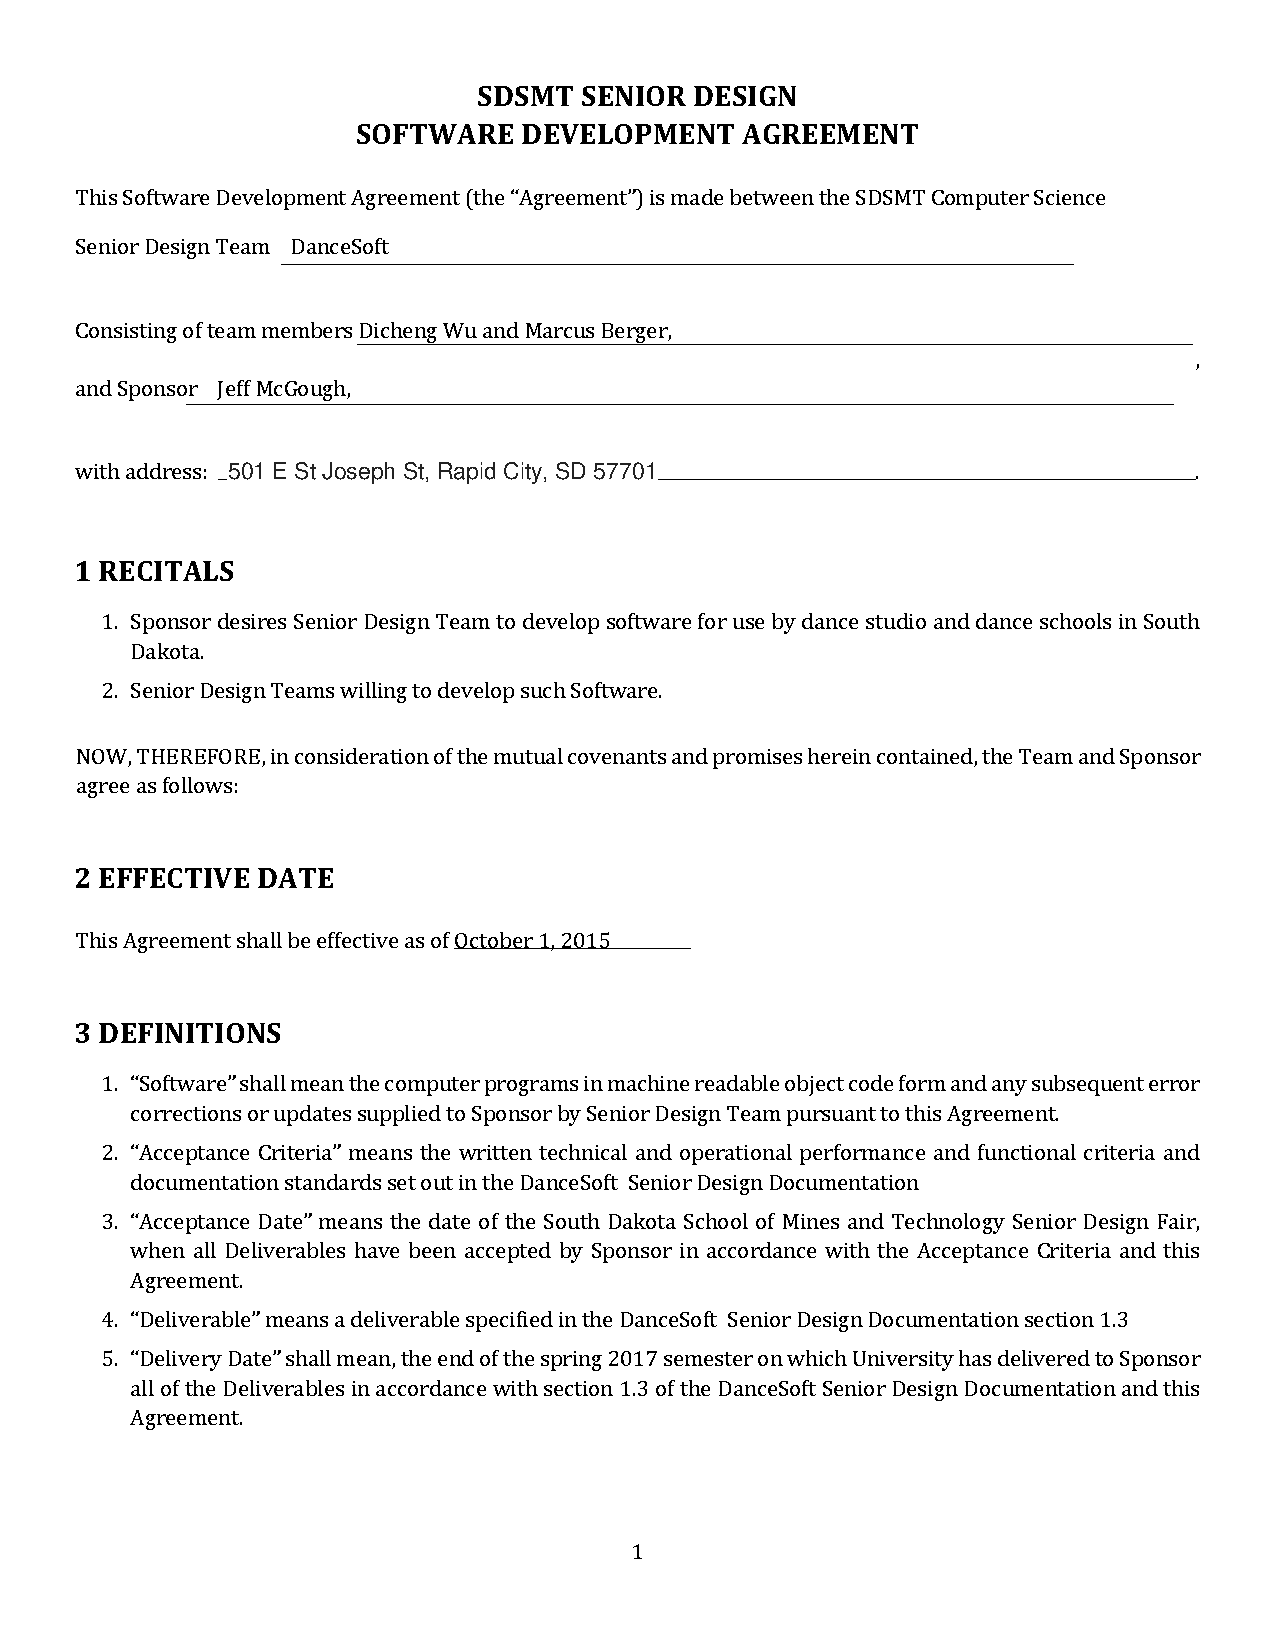
\includepdf[pages={1-5}]{SoftwareContract.pdf}

% In our style file, appendices are numbered with capital letters
\appendix

\chapter{Product Description}

	The DanceSoft product developed by the South Dakota School of Mines and Technology senior design team of Marcus Berger and Dicheng Wu is a proof of concept for an administrative software to run the day to day activities of the Rapid City Academy of Dance Arts. The teams overall goal is to provide a proof of concept to the client Dr. Jeff McGough, to show that a viable software is indeed possible to meet the needs of the Academy and eventually through continued iteration by other senior design groups or by outside entities the project will replace the software currently in use at the Rapid City Academy of Dance Arts\\
	
	The product will demonstrate a set of core functionalities that will be used to run the Academy, these functions include adding students, and teachers, assigning classes to teachers, registering students, ability to produce schedules and roll sheets, and a very rudimentary billing system that will be a blueprint for future iterations of the software.  Other functions needed to complete this core functionality are also included in the system. 
The projects provides an admin interface where the teachers who are registered as admin can do several data manipulation task for the system. These task include managing classes, students and teachers, updating Academy personal information, and dealing with a simple billing system. The project also provided a teacher interface where teachers registered in the system are able to manage their needs. Teachers are able to view student information such as name, guardian, address, and emergency contact. Teachers are also able to search classes, produce student and teacher schedules, and produce class role sheets. Lastly teachers are able to modify their personal information, this includes a form to change fields such as address, and medical information, and the user can also modify name, date of birth and other field should mistakes be made when the teacher is first entered. Also the teacher is able to change their log in credentials and enter their hours for viewing by system admins.\\

	As a proof of concept this software is meant to give the client a minimum viable product, or more likely provide a blueprint for a future system iteration whether that be a future senior design project, or a contract software. In accordance with the clients request this product is not meant to be an industrial software at the completion of the senior design project. The overall goal remains to give the client an idea of the possibilities of a full industrial Academy of Dance Arts software.


\vspace{2\baselineskip}




\chapter{Sprint Reports}
% !TEX root = DesignDocument.tex


\section{Sprint Report \#1}
Sprint Report \#1


\subsection{Team Members:}
Dicheng Wu
\\Marcus Berger\\
\textbf{Sponsor:}
\\Jeff McGough
\\

\subsection{Customer description}

\subsubsection{Description of sponsoring customer}
The sponsoring customer for this project is Dr. Jeff McGough a computer science professor at the South Dakota School of Mines and Technology and the vice president of the Academy of Dance Arts in Rapid City, South Dakota. Well not the sponsor of the project Dr. McGough's wife is also a key part of the customer base as the owner of the Academy. She and other dance school owner are the target group for this project. 

\subsubsection{Statement of customer's problem or goal for this project}
The customer wants a software that can run the day to day operations of a dance studio and also handle record keeping, billing, payroll, and other business operations
 
\subsubsection{Customer's Needs}
The customer needs us to develop a software solution which can run the dance studio in an effective manner. The product also needs to handle changing classes from year to year without needing to be updated. This means that the software needs to sync with multiple users, and handle new information such as class rosters, prices, clothing requirements for classes, changes in the employment roster, and many other changes that can occur in the running of a dance school.\\
This project as a whole needs to be an improvement on the current system in use by the customer and provide an easy and efficient way to run the clients business. 



\subsection{Overview of the project:}
The project consists of three major parts, GUI, database and back end code. For the Gui part, we are going to integrate everything into a small number of windows to eliminate the need for large numbers of window like the current product in use at the academy. and, thus, users can manipulate it very straightforwardly. For database part, we are going to build a database which stores students, employees, classes, billing, and other information needed for the academy to function as a business. For the code back end, we are going to develop it on using Python and PyQt with a primary focus on Mac but with cross platform compatibles. 

\subsection{Project Environment:}

\subsubsection{Project boundaries}
The boundaries of this project would be the Academy of Dance Arts in Rapid City. The product could be used by other dance schools in the future but they are out of the scope of this projects development 

\subsubsection{Project context}
The context of this project is only to develop a better software solution to the current software in use at the Academy of Dance Arts in Rapid City, South Dakota, so they can run their school in a more efficient manner. While the project is open source it is not the intention of this team to develop an all purpose solution for all the dance schools around the country. This project is tailored to the needs of the Academy of Dance Arts.


\subsection{Project deliverables of Sprint 1:}

\begin{enumerate}
\item The research into program languages, database and GUI frameworks and architectures for the DanceSoft project.
\item Final decision on frameworks and architectures for the DanceSoft project.
\item User Stories and Product Backlogs for the project.
\item Creating a very simple Qt window.
\end{enumerate}

\subsection{User Stories}

After the requirement for the project were laid out the team created the user stories based on those requirement. The user stories the team came up with are as fallows:

\begin{enumerate}
  \item As a user i want to adjust students payment models
  \item As the owner I would like to see automatic database backups.
  \item As a student I would like to be able to register online (with special app). Classes must be approved before added.
  \item As a student I would like to be able to search clothing requirements.
  \item As a student I would like to know my billing.
  \item As the owner I would like to indicate clothing requirements per class.
  \item As a studio person, I would like to be able to add students to classes.
  \item  As a student, teacher etc, I would like to be able to look up a students class list.
  \item As the teacher I would like to get a class role for each class.
  \item Given a class list, I would like to get an invoice of the tuition due.
  \item Studio would like to track payments and estimate remainder due.  I would like to generate an invoice for this amount.
  \item As a student I would like to be able to register online (with special app).   Classes must be approved before added.
  \item As a student I would like to know my billing.
  \item As the owner I would like to track teacher hours and compute payroll.
  \item As the owner I would like to indicate clothing requirements per class.
  \item As a student I would like to be able to search clothing requirements.
  \item As the owner I would like to see automatic database backups.
\end{enumerate}

\subsection{Product Backlog:}

From the above user stories the team produced the fallowing product backlog. The parts are not in the order of execution. More thing will be add or removed to this in the future as the software develops.

\begin{enumerate}
\item Create the database tables
\item Create database backup system
\item Create online register page and approval system
\item create clothing requirement update function, and add clothing function for teachers and admin
\item create clothing viewer function for students
\item create dynamic billing algorithms (expand on later sprint)
\item create page for tuition calculation and viewing by students
\item Add and subtract students from a class
\item Create dynamic Queries to produce class attendance list
\item Hour tracker for teachers and payroll calculation algorithm (expanded later)
\item Using dynamic DNS service to set up Linux Box
\item Encrypt data that store in the database
\item retrieve data from database to produce a invoice for payroll
\item queries in database to retrieve student information
\item Create ability for employee to look up and modify student registration info
\item Query database to produce class role sheet
\item Query database to produce employee information
\item create permission assignment system
\item handle billing info (expand later)
\item Create dynamic algorithm for payment model creation and calculation. 
\item Algorithm for payment tracking and remainder calculation, and query database to produce invoice.
\item Query and insert information needed to create and new class and produce a results page.
\item Create update query to assign teachers to a class
\end{enumerate}

\begin{figure}
\caption{DanceSoft Trello Board}
\centering
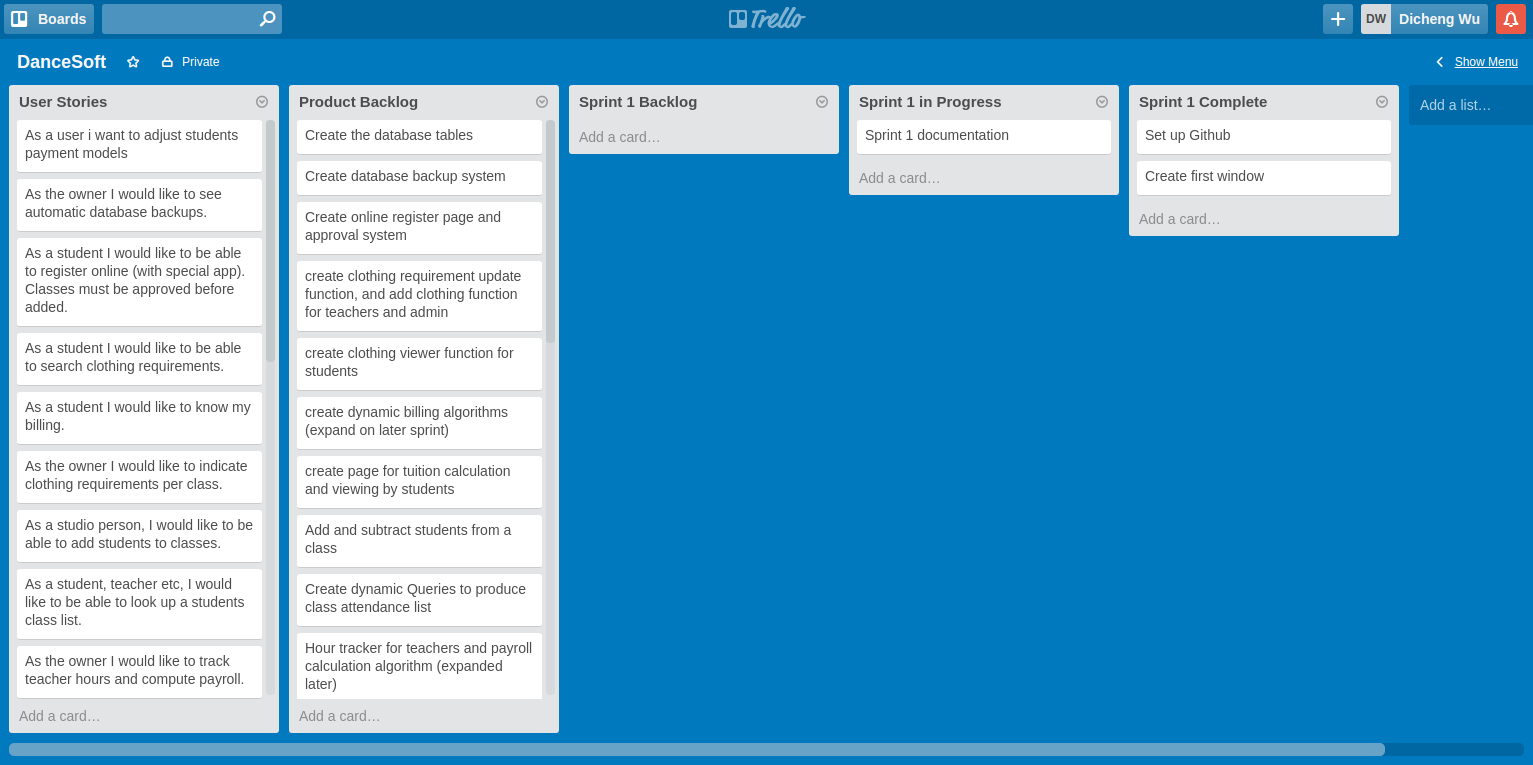
\includegraphics[width=0.5\textwidth]{d1}
\end{figure}



\subsubsection{Sprint 1 Backlog:}

\begin{enumerate}
\item Set up Github
\item Design Research
\item Design Decision
\item Create first window
\item Sprint 1 documentation
\item Sprint 1 Review
\item Continuing practice with QT

\end{enumerate}

\subsection{Research}

\subsubsection{Database Research}

\subsubsection{SQL VS NonSQL:}
SQL is designed for fixing data structure and the scale of amount of data in database should be medium size otherwise with it growing big the database will drop down its speed. NonSQL is designed for frequent changing data structure and the scale of amount of data in database does not affect the performance of the database a lot. The SQL database is stable and however the NonSQL is constantly suffering fail overs. The database aims to store employees and students and classes information and the size of students less than 4000 and the size of employees less than 10. The structure of data is stable, by considering all those facts above, we decide to use SQL database.\\

\textbf{The different SQL Databases:}\\
For this part, we think of using MySQL. MySQL is a free software and widely used in different fields. It has a very good portability and can runs over different OS systems and aims for small size of data. Also our experience is more focused in MySQL, and the feature set for SQL in MySQL fits within the scope of the project, for these reasons we choose MySQL as the database frame work.

\subsubsection{Storage Options:}
For this part, We considered three options, local, cloud, mixed. Since the database is accessed by different devices and the internet in the Academy is not stable, we decide to use mixed storage schema either Amazon AWS plus a local database or a Linux box plus a local database. After researching Amazon AWS, it does not support storing images and videos which the Academy may require in the future, therefore   due to some inconsistency in the internet and the current and possible future needs of the Academy we decided to go with a local Linux box and database.\\

\subsubsection{Languages}
Since the Academy is currently running a Mac system the first language idea was objective-C. Recently though Apple released a programming language update called Swift. Due to our teams inexperience with Mac and the possibility of the dance academy being sold in the future we were faced with a choice, between Python or Swift. Swift is a c++ like language which stuck out as a possible jumping off point for us. However as we researched it became clear that swift would have a high ramp up time and learning curve. On top of this as novices to the Mac development environment we would spend a large amount of time just trying to figure out the system. As far as pluses for Swift the language has all the functionally of objective-C plus things added to make the language better, overall reception for the language within the Mac community have been positive. The language itself is designed with porting to IOS in mind which would make a mobile transition more likely. The language would use Cocco as a GUI environment which is also relatively well revived by OSX developers, ut again ramp up for our team would be high.

The language competing with Swift in our discussions was Python. Python has the upside of being a language the team is more experienced in. Also the client Dr. McGough knows Python so any updates would be easier for him to do. Python is also a cross platform language which allows the team to produce working code for Mac, Windows, and Linux at the same time and on any operating system. This means the the team can develop on Windows or Linux, development environments we are more familiar with, and have the code work on Mac. Also development in Python means that if the academy was ever sold to a Windows user the product would still work. Another advantage we discovered to python is the academic and career experience it provide since in our research for the SD Mines career fair we discovered that many companies use Python and more than expected would like QT experience. Lastly the Python community is larger and can more readily provide assistance if needed through websites and research.

So overall while Python is not Mac native it provides more viable reasons for use in our teams eyes. That is not to say we don't believe Swift is a good choice, Swift is a completely viable choice for a product like this it is just not the best for the exact situation the team is in. So we have decided to create the  Academy of Dance Arts Software in Python using PyQt as a GUI. 

\subsection{Final Framework Decision}
Language: Python\\
Gui: PyQt\\
Database: Mysql\\

\subsection{Foreseeable issues}
As of the sprint 1 review, possibly issues could include database encryption and synchronization, team learning curve of Qt.\\
\\
  

\section{Sprint Report \#2}
Sprint Report \#2


\subsection{Team Members:}
Marcus Berger
\\Dicheng Wu\\
\textbf{Sponsor:}
\\Jeff McGough
\\

\subsection{Prototype Progress}
The progress is mostly out of the research phase and has began the first steps of production. The progress is laid out in more detail in this report. As of now the prototype is in a state to begin working on functionality. The rough (not final) GUI pages are laid out and being constructed to give us an environment for creating the functionality. The back end database has been constructed and will allow us to begin testing the database connected page as we create them. Current pages constructed are log in page, landing pages, and some options page.

\subsection{Project deliverables of Sprint 2:}

\begin{enumerate}
\item The database creation script  
\item Gui path work, meaning figuring out the path through the Gui architecture 
\item Log in page that reads users permission level and sends them to the correct landing page
\item Rough landing pages for Admin and Teachers (design improvements to come in later sprint) 
\end{enumerate}


\subsubsection{Sprint 2 Backlog:}

\begin{enumerate}
\item Creation of database tables 
\item Draw GUI path
\item Decision on rough GUI theme
\item Create a log in page that sends the user to the correct landing page based on their permission level
\item Create rough versions of teacher and admin landing pages to test functionally (improve look in latter sprint 
\item Continue rough GUI page creation to have environments for functionality 
\item Sprint 2 Review
\item Continuing practice with QT
\end{enumerate}

\subsection{Database Creation}

The first thing we tackled in sprint 2 was getting the database up so we could begin actually developing the product and give our qt interface something to actually interface with. The main goal here was to make sure we had constructed the database in such a way that it could complete all the user stories it needed to in a way that made sense. After talking through the tables and the users stories we came up with the table creation script that was submitted with this sprint. While modifications will need to be made for when we do the billing side of the project, we think that this table structure should provide for the need of the academy.

A few thing to note in the database, we created student\_class and teacher\_class tables to deal with the many to many relationships in the database. Also there are no payroll or transaction tables yet as the group is still trying to figure out how to handle billing information and data.


\begin{figure}
\caption{Tables currently in database}
\centering
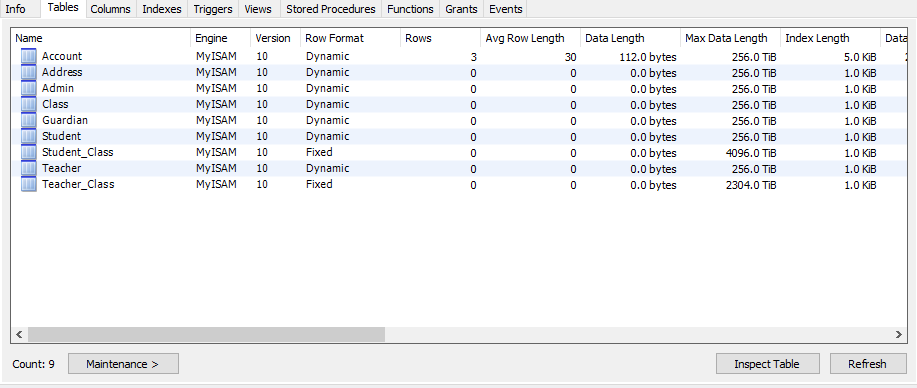
\includegraphics[width=0.5\textwidth]{database_tables}
\end{figure}

\subsection{GUI Work}

\subsubsection{GUI Path and Theme}

The path for the gui was part of the backlog so we could figure out the minimum number of pages we would need to do the things required by this project. This does not mean we are looking to create only the minimum but just get a general idea of how many pages we would need. Also it allowed us to see how the pages were connected and how we expect navigation through the system to work. The rough drawing of the path can be found in the Github repo's sprint two folder.

The other thing we need was to talk to the client about what he wanted for a navigation theme. We came up with three options, first was a button layout on the top and side of the page, second was  drop down menu similar to the way was mac and windows handle navigation in their products. Last was an expanding folder structure similar to that of the content management system Ektron. After consulting with Dr. McGough, he  decided that the more familiar drop down menu would be the easiest and most user friendly option and the option he would prefer we do. This decision allows us to use the built in menu bar functionality of PyQt and should reduce work load on navigation for this project.

Another part of theme is color and design, the color scheme will most likely resemble the academy's color plate, but the improve design will be worked on later. As of now the primary focus is making sure all the functionality works.


\subsubsection{GUI Pages}

The GUI pages for this sprint were the log in page and the landing pages for admin and teachers. The student part of the gui will be php which will be worked on in a future sprint once the functionality is done. Since the student functions are similar to some of the admin or teacher functions most work should port over fairly quickly.

The first page we made was a log in in page that takes a user name and a password and first checks to see if they exist and are correct within the system. If they are not a dialog saying whats wrong appears and prompts the user again. If the information passes the check the system reads the users permission level and sends them to the corresponding landing page.

\begin{figure}
\caption{Current iteration of the log in page}
\centering
\includegraphics[width=0.5\textwidth]{login_page}
\end{figure}

The other set of pages we need to make to begin writing functionality was the landing pages for the admin and teacher permission levels. These pages show the types of things each can do and allow navigation to the various different functionality that permission level can do. For example the admin landing page has a button to take you to a student options page, from there you select which option you want and will be taken to the page to execute that function. The idea is to start at the landing page and be able to navigate to a specific function in three or four clicks max. The menu bar will also execute navigation and should allow the user to jump to a desired function.\\

\begin{figure}
\caption{Current iteration of the Admin Landing page}
\centering
\includegraphics[width=0.5\textwidth]{admin_landing}
\end{figure}

Pages currently being worked on include:

\begin{enumerate}
\item Search pages
\item Modify data page
\item Add information and new information pages
\end{enumerate}


\subsection{Sprint 2 Issues}
Some issues that were encountered during this sprint were:

\begin{enumerate}
\item Running out of time - the group found it hard to complete this sprint on time due to many time draining issues, such as other class work,family matters, midterm exams and a client presentation during this sprint. Mitigation for this issue will be better time management for the team.
\item Inexperience with PyQt - The team ran into some issues that drained on time when working with PyQt, such as looking up information on how to perform a needed task. Mitigation for this issue is mostly experience based as we learn the system and learn how to more efficiently navigate the community the time sink should go down.
\item Team communication - The team found some issues in communicating with one another because of the language barriers within the team. Which in some cases slowed sprint progress. Mitigation for this issue will come with time as the group begin to understand each other better and find efficient patterns of communication.
\end{enumerate}

\subsection{Client Interactions}

Client interactions came in the form of weekly meeting every wednesday at 2:00 p.m. Topics included:

\begin{enumerate}
\item Progress reports on where we are in the project
\item Asking questions to refine functionality and understand academy needs
\item Discuss the future of the project and idea on how to execute them
\end{enumerate}


\subsection{Group Meeting}

The group has a standard meeting time of 4:00-5:00 or 4:00-6:00 MWF and a second meeting time of TTH 10:00 - 12:00

Meeting can continue pass these times if needed, and other times during the weekend. However weekend times fluctuate and do not remain constant from week to week. 

\subsection{Work Distribution}

Marcus:
\begin{enumerate}
\item GUI Path Charts
\item Landing page Construction\\
\end{enumerate}

Dicheng:
\begin{enumerate}
\item GUI Theme Ideas
\item Log In Page and Permission Navigation\\
\end{enumerate}


Together:
\begin{enumerate}
\item Wrote and talked through database and construction
\item Got database running
\item GUI page breakdown based on user stories and product backlog
\item Coded some functionality
\end{enumerate}


\section{Sprint Report \#3}

Sprint Report \#3


\subsection{Team Members:}
Marcus Berger
\\Dicheng Wu\\
\textbf{Sponsor:}
\\Jeff McGough
\\

\subsection{Prototype Progress}
The progress is being made on the simpler functions of the projects including search, updates, and role sheets. As of now the prototype is in a state of some working functionality on the admin and teacher side. The pages are not yet tied together but the complete functions function independently. Several GUI pages are complete or in a working state to compliment these functions. The back end database has been slightly updated to adjust to the needs of the project. Lastly the prototype has reached a state where testing can be conducted on parts of the project, more information is given later in this document.

\subsection{Project deliverables of Sprint 3:}

\begin{enumerate}
\item Student search page 
\item Employee search page
\item Add a class to the database
\item Update teacher and student information pages
\item Modify clothing requirements for a class
\item Generate a class role sheet
\item Assign teacher to a class
\item Ability to add and subtract students from a class  
\end{enumerate}


\subsubsection{Sprint 3 Backlog:}

\begin{enumerate}
\item Queries in database to retrieve student and employee information
\item Query and insert information needed to create and new class and produce a results page.
\item Query database to produce class role sheet
\item Create clothing requirement update function, and add clothing function for teachers and admin
\item Create update query to assign teachers to a class
\item Create ability for employee to look up and modify student registration info
\item Add and subtract students from a class
\item Sprint 3 Review
\item Create Client presentation
\item Documentation for semester
\end{enumerate}

\subsection{Search Pages}
The first page tackled this sprint was the search page. The page takes user input and searches based on name using a fuzzy search. Also included in both searches is an advanced search option that allows the user to check boxes corresponding to the fields in the database, which allows the user to search in more versatile ways. Lastly the user can click on a student to pull up all of their information and modify it as needed.


\begin{figure}
\caption{Search Pages}
\centering
\includegraphics[width=0.5\textwidth]{search.png}
\end{figure}

\subsection{Add A Class}
Clicking on the "Add a Class" button on the admin landing page will open a dialog. From this dialog box the user can type in information to a add a class. These fields include class name, cost, start and end times, day, clothing requirements, class description, start and end dates, and the age range for the class.  At the time of class creation only name, is a required field. When the submit button is clicked a message box will pop up to confirm the database submission before submitting to the database  

\subsection{Role Sheet}
This page generates a list of classes teachers are currently teaching. Teacher can see who is taking his/her class by selecting the corresponding class on the list and can print this list as a pdf. 

\subsection{Update Pages}
These pages are fairly simple to explain sometimes the user will need to add or alter a record of some kind these pages need to be able to do that in a simple and concise way. The update pages worked on in this sprint include student information from the employee side, updating teacher information and updates to clothing requirements for a class. Most of these page will just produce a form where information can be displayed and updated.

\subsection{Assign Teacher to a Class}
This page allows an admin to select a class, clicking on a class pulls up a list of available teachers to select to teach the class. Clicking on a teacher will pull up a message box to confirm the selections before submitting to the database. The available teachers are selected based on the start time of the selected class and the end time of the classes already being taught by each teacher. If the class times overlap then that teacher will not show up in the available teachers list.

\subsection{Sprint 3 Issues}
Some issues that were encountered during this sprint were:

\begin{enumerate}
\item Time - While not as much of a problem as it was in sprint two the group still found itself running low on time. The lead gained during Christmas break should reduce the issue in phase 2.
\item Inexperience with PyQt - While still a small issue the experience of the team is growing and while some issues still exist such as needing to look up information at times, the issues are lessened from the last sprint.
\item Team communication - The team found some issues in communicating with one another because of other projects and assignments. Which in some cases slowed sprint progress. Mitigation for this issue will be to more strongly impose a schedule in phase 2.
\end{enumerate}

\subsection{Client Interactions}

Client interactions came in the form of weekly meeting every Wednesday at 2:00 p.m. Topics included:

\begin{enumerate}
\item Progress reports on where we are in the project
\item Asking questions to refine functionality and understand academy needs
\item Discuss the future of the project and idea on how to execute them
\end{enumerate}


\subsection{Group Meeting}

The group has a standard meeting time of TTH 10:00 - 12:00 and once during the weekend usually from 1:00-5:00 

Meeting can continue pass these times if needed, and other times during the weekend. However extra weekend times fluctuate and do not remain constant from week to week. 

\subsection{Work Distribution}

Marcus:
\begin{enumerate}
\item Add a class
\item Assign teacher to class
\item Update teacher page
\item Update clothing
\item Documentation
\item Trello management\\
\end{enumerate}

Dicheng:
\begin{enumerate}
\item Search Pages
\item Role sheet
\item Modify student information
\item Add and Subtract students from a class
\item Navigation to teacher or admin page\\
\end{enumerate}


Together:
\begin{enumerate}
\item Updated database construction
\item GUI page breakdown based on user stories and product backlog
\item Coded some functionality
\end{enumerate}

\section{Sprint Report \#4}

Sprint Report \#4


\subsection{Team Members:}
Marcus Berger
\\Dicheng Wu\\
\textbf{Sponsor:}
\\Jeff McGough
\\

\subsection{Prototype Progress}
During sprint 3.5 the team organized the functionality and tied them together to create the single current working prototype. Other updates were made to fix known bugs and add a class search. While the team worked on putting the project together smaller bugs or needed pages that were implied by user stories were tackled as they came up. This resulted in to much time being used, so the student interface was not tackled. The student interface has since been dropped from the clients project requirements due to time.

Sprint 4 was dedicated to payroll and billing. First the client rewrote the user stories to provide more clarity to the team. After this the user stories were tackled by the group to produce the first draft of the payroll and billing interface. This included logging hours, payments, fees, rates, credits, and discounts. After this was done the team demoed the project for the client and got notes on the project as a whole. These notes will be tackled as part of the backlog in the next sprint.


\subsection{Project deliverables of Sprint 3.5 and 4:}
Sprint 3.5 had no defined deliverables, and was mostly clean up.

Sprint 4 deliverable was the first draft of the payroll and billing interfaces and functions, layed out in the user stories below.



\subsubsection{Sprint 3.5 Backlog}

\begin{enumerate}
\item Fix Assign Teacher to Class Dialog Bug
\item Add Class Search
\item Complete Role Sheet
\item Tie Functions Together
\item Fix Smaller Bugs
\end{enumerate}

\subsubsection{Sprint 4 Backlog:}

\begin{enumerate}
\item View Teaching History
\item Look at The Current Amount Someone Owes
\item Generate an Invoice For The Amount Due
\item Look at Billing History
\item Apply Credits to a Students Account
\item Enter the Tuition and Fees Rate
\item Give Early Registration Discounts
\item Enter Staff Pay Rates
\item Enter a Full Payment for One Student 
\item Enter a Full Payment for Several Students
\item Enter Payments From Multiple Sources For One or More Students
\item Compute Teacher Wages 
\item Enter Staff Hours
\item Give Prorated Refunds 
\end{enumerate}

\subsection{Sprint 3.5}
During sprint 3.5 Class Search was added this page follows the same format as other search pages created in previous sprints. Also completed fixes to the assign teacher to class bug, role sheet completeness, and a few other minors bugs. At the end of the sprint the team tied what we had together so the product could run as a unit starting from the log in screen.

\subsection{Prorated Refunds}
The prorated refunds code will keep track of how much a class costed a student. If the student drops a class it will refund the remaining worth of the class to the students school credit field. This file is still in progress.

\subsection{Enter Staff Hours}
This page needs to undergo changes after meeting with client. The new version will allow a teacher to log their in class hours, office hours, trip hours, etc. These hours will then be paid out at their different rates respectfully. The hours will be logged as single numbers not by days or weeks.

\subsection{Enter Teacher Wages}
This was handled in the database in previous sprints assuming one pay rate. However in talks with the client the academy pays different pay rates based on what part of academy work they are doing. So the page will need to be updated once the list of possible pay rates have been provided by the client.

\subsection{Enter Tuition Rates and Fees}
These pages allow the user to look at the current tuition rates and fees. The user can then update existing rates, add new rates, or remove rates that are no longer needed. Tuition rates are logged in the database as flat minute rates. The user can enter new rates in the form of minutes or hours.

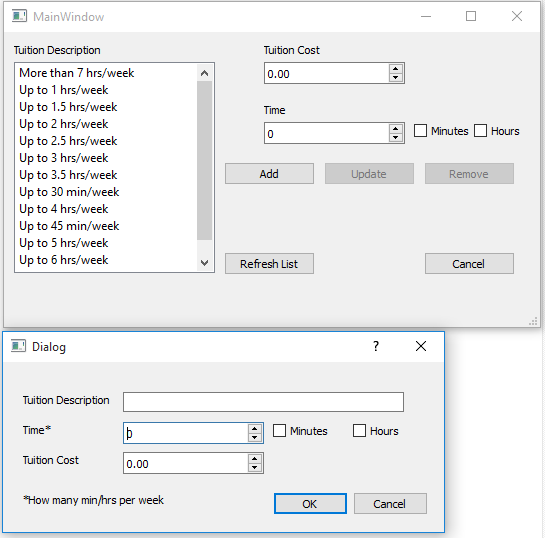
\includegraphics[scale=0.5]{tuitionRates.png}

\subsection{Teacher History}
This page includes several components. Firstly, user can use this page to find a specific teacher by entering a full or partial name of teachers. Secondly, users can click the history button to open up another window which has a list of classes the teacher has taught.\\

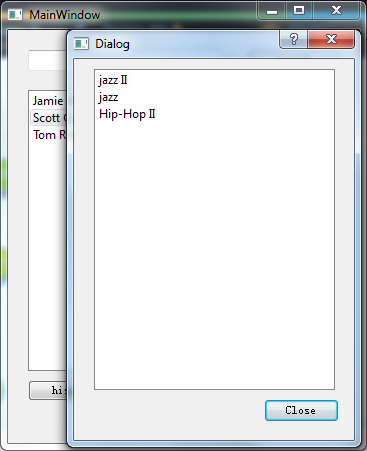
\includegraphics[scale=0.5]{teacherHistory.png}

\subsection{Set Semester}
This page helps users to set the current semester from pool of semester and add a new semester to the system.

\subsection{partial payment}
This page includes several components. Firstly, user can use this page to find a specific student by entering a full or partial name of students. Secondly, users can click the pay button to open up another window which asks user to input amount of money paid, payment's method and semester paid. The user also can choose single or multiple students at one time. \\
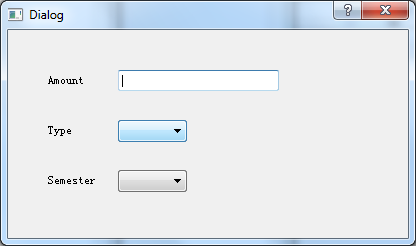
\includegraphics[scale=0.5]{payment.png}

\subsection{Student's owe}
This page includes several components. Firstly, user can use this page to find a specific student by entering a full or partial name of students. Secondly, users can click the statement button to open up another window which shows the amount of students paid, the amount of students due and the balance of student's account. Users also can print the invoice generated by the window.\\
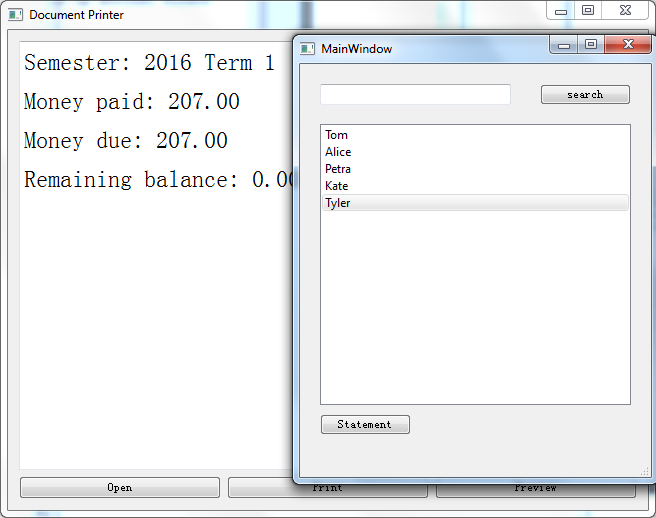
\includegraphics[scale=0.5]{invoice.png}

\subsection{enter payment}
This page includes several components. Firstly, user can use this page to find a specific student by entering a full or partial name of students. Secondly, users can click the clear button to clear the due of selected students. Users can select single or multiple students at one time.\\
\includegraphics[scale=0.5]{enterPayment.png}

\subsection{bill history}
This page includes several components. Firstly, user can use this page to find a specific student by entering a full or partial name of students. Secondly, users can click the statement button in order to get the list of payments. In addition, user can print the bill history.\\

\includegraphics[scale=0.5]{billHistory.png}

\subsection{Sprint 3.5 and 4 Issues}
Some issues that were encountered during this sprint were:

\begin{enumerate}
\item During winter break the team wanted to tackle the student interface app. Building other required pages in the main local GUI made this a problem. Therefore while some implied GUI pages where fixed and created, the team was unable to get to the student interface. As a result the student interface was removed from the project requirements.
\item Spring semester ramp up - Coming back from a month break meant that the team needed to ramp back up and get used to the new classes and new commitments. This cause the team to move slower then it should have in this sprint. 
\item Team communication - The meeting this sprint were less effective as teams members would have other commitments, or in some cases lack the drive to do the work. This lessen as the sprint continued, but sometimes still came up.
\item Requirement Confusion - At times during this sprint the requirement were confusing. This resulted in a rewrite of the requires for payroll and billing to provide more clairity and adjust for dropping the student interface. The rework helped the team greatly, however the user stories still sometimes left out core part of how the academy does its work compared to other places. This resulted in spending more then the usually time speaking with the client, and group friction.
\end{enumerate}

\subsection{Client Interactions}

Client interactions came in the form of requires reviews and a demo of the prototype at the end of the sprint. Topics included:

\begin{enumerate}
\item Progress reports on where we are in the project
\item Asking questions to refine functionality, understand academy needs, and update requirements.
\item Discuss the future of the project and idea on how to execute them.
\item Prototype the current version of the prototype.
\end{enumerate}


\subsection{Group Meeting}

The group has a standard meeting time of TTH 10:00 - 12:00 and once during the weekend and at home as needed.  

Meeting can continue pass these times if needed, and other times during the weekend. However extra weekend times fluctuate and do not remain constant from week to week. 

\subsection{Work Distribution}

Marcus:
\begin{enumerate}
\item 3.5 Fix Assign Teacher Bug
\item 3.5 Update GUI Functions, Minor Additions and Fixes
\item 3.5 Tie Various Functions Into a Single Prototype
\item Prorated Refund (Still in Progress)
\item Enter Teacher Hours (Still in Progress)
\item Teacher Pay Rates (Needs Updated With New Information)
\item Early Registration Discounts
\item Gives Credits
\item Enter and Update Tuition Rates
\item Enter and Update Fee Rates and Type (Needs Updated With New Information)
\item documentation
\item Trello management\\
\end{enumerate}

Dicheng:
\begin{enumerate}
\item 3.5 Tie function together
\item 3.5 Class Search Pages
\item 3.5 Updated Role sheet
\item 3.5 Research Linux Boxes
\item 3.5 Tie Functions Together Into a Single Prototype
\item Enter Payments From Multiple Sources For One or More Students
\item Look at The Billing History
\item Enter a Full Payment For One or More Students
\item Enter Payments From Multiple Sources For One or More Students
\item Generate an invoice for the amount due (Needs Updated)
\item Look at a The Current Amount a Student/Family Owes
\item View Teaching History
\item Auto and Manual discount giving
\item Set semester
\end{enumerate}


Together:
\begin{enumerate}
\item Updated database construction
\item GUI page breakdown based on user stories and product backlog
\item Coded some functionality
\end{enumerate}

\section{Sprint Report \#5}

Sprint Report \#5


\subsection{Team Members:}
Marcus Berger
\\Dicheng Wu\\
\textbf{Sponsor:}
\\Jeff McGough
\\

\subsection{Prototype Progress}


Sprint five was dedicated to finishing the last of the functions and clean up of the project. First the client modified  some requirements for the team. After this the user stories remaining from sprint four were tackled by the group to produce the remaining payroll and billing interface. This included logging hours, and payments. After this was done the team started on bug fixes and quality of life updates such as new buttons and removal functions. The team is currently working on finishing up the student registration. If progress continues at this rate the prototype should be completed functionally for our teams iteration however without some work the prototype may not reach some of the teams desired standard.


\subsection{Project deliverables of Sprint 5:}

Sprint 5 deliverables were the remaining functionality for the redefined requirements from the client for the project. If the sprint was successful the main project will be done or very close to done functionally for this iteration at the end of the sprint.


\subsubsection{Sprint 5 Backlog}

\begin{enumerate}
\item Admin and teacher update crossover
\item Ignoring case in address forms
\item Add rejected students to approved/ reject and provide current status
\item Multiple pay rates
\item Admin list function
\item Enter staff hours
\item Sprint 4 rollover (remaining payroll functions)
\item Add and remove class location
\item Removal Functions (Admin, Class, Student, Teacher)
\item Refunds and check boxes for fees and tuition
\item Quality of life updates to some functions
\item Bug Fixes
\item Student registration
\item Employee wages
\item Begin User Guide for documentation
\end{enumerate}


\subsection{Sprint 5}
During sprint five the team tackled the remaining functionally, bugs, and quality updates in an attempt to finish the base project. Removal functions to clean out the database were added, and some client requested quality of life updates were added for this project version. Bugs and glitches were patched up in many functions. Another job of this sprint was to finish the rollover from sprint four since some payroll functions still needed work. Lastly the team tackled student registration since the student interface was dropped from the project requirements in sprint 4. The registration is still in progress at this time, as the team failed to complete this functionality in time for the end of the sprint. However it was completed during sprint 6.

\subsection{Prorated Refunds}
The prorated refunds code will keep track of how much a class costed a student. If the student drops a class it will refund the remaining worth of the class to the students school credit field. This file has now been completed.

\subsection{Enter Staff Hours}
This page needed to undergo changes after meeting with client. The new version will allow a teacher to log their in class hours, office hours, trip hours, etc. These hours will then be paid out at their different rates respectfully. The hours will be logged as single numbers not by days or weeks. This function is now completed

\subsection{Enter Teacher Wages}
This was handled in the database in previous sprints assuming one pay rate. However in talks with the client the academy pays different pay rates based on what part of academy work they are doing. So the page will need to be updated once the list of possible pay rates have been provided by the client. This pages and its updates are still in progress. \\

\includegraphics[scale=0.5]{payRates.png}

\subsection{Enter Tuition Rates and Fees}
Updated these pages to provide quality of life updates to the function requested by the client.\\

\includegraphics[scale=0.5]{feeDialog.png}

\subsection{Bug Fixes}
During the course of testing and the client meeting some bugs or inconsistencies were discovered within the project. The bugs found and fixed are:

\begin{enumerate}
\item Student search was not showing all the students. Status: Fixed
\item Search edit need to be turned off and advance search modifications. Status: Fixed
\item Search, role, and schedules need to have dynamic not static times. Status: Fixed
\item Allow for time changes on schedule. Status: Fixed
\item Some of the back buttons in the teacher interface did not work correctly. Status: Fixed
\item Forms seem to be bugged at times, however can not recreate bug. Status: In testing possibly fixed.  
\end{enumerate}

\subsection{Updates Crossover}
One of the updates that needed to be completed this sprint was the need for admin and teacher updates to crossover if something was changed. This means that if someone is an admin and they update there phone number through the "update my information form" then the phone number will be updated in both the teacher table and the admin table. This way the system will not have conflicting information in different places. 

\subsection{Approved/Rejected Student Updates}
A update requested by the client was the ability to see rejected students in the approved/rejected pages just in case the academy changed its mind about a student. The page underwent slight modifications to the way information was displayed to make this change efficiently\\

\includegraphics[scale=0.5]{newAddStudent.png}

\subsection{Admin List}
In creating some of the updates it became clear that a specific admin list was needed to see who had admin access to the system. This was done through a simple list view of the names that can then be selected to display more detailed information.\\


\subsection{Add/Remove Locations}
Another requested feature was the ability to add and remove locations for classes in the database. This feature is necessary because the academy sometimes teaches classes in different places based on need. The team accomplished this using a simple dialog that connects to the location table in the database. When the user updates or adds a new class the location combo box provides a list of locations in the database and an add location option.\\

\includegraphics[scale=0.5]{newLocation.png}


\subsection{Removal Functions}
These are simple functions that pull up a dialog box where the user can select a name and remove all the information related to that user from the system. The removal functions that exist in the system are: teacher, admin, student, and class. Teacher will remove that persons information from the system. Admin removes that persons admin rights and then ask if the whole user should be removed.\\

\includegraphics[scale=0.5]{removal.png}

\subsection{Sprint 5 Issues}
Some issues that were encountered during this sprint were:

\begin{enumerate}
\item Spring semester ramp up - This was by far the biggest issue this sprint and the main cause of the failures this sprint. Other classes  up to the point of blocking work on many projects. Staggered due dates meant that when the team wanted to work, there was always another projects that needed to be completed in a short amount of time. By the end much of our time had been taken and the sprint began to fall behind.  
\item Requirement redefining - Due to drop the student interface the functionally needs to be added to the GUI which created some extra work for the team. 
\item Failure to complete backlog - The team did not finish all of the assign backlog this sprint.
\end{enumerate}

\subsection{Client Interactions}

Client interactions came in the form of required reviews and a demo of the prototype at the end of the sprint. Topics included:

\begin{enumerate}
\item Progress reports on where we are in the project
\item Asking questions to refine functionality, understand academy needs, and update requirements.
\item Discuss the future of the project and idea on how to execute them.
\item Prototype the current version of the prototype.
\end{enumerate}


\subsection{Group Meeting}

The group has a standard meeting time of TTH 10:00 - 12:00 and once during the weekend and at home as needed.  

Meeting can continue pass these times if needed, and other times during the weekend. However extra weekend times fluctuate and do not remain constant from week to week. 

\subsection{Work Distribution}

Marcus:
\begin{enumerate}
\item Bug fixes
\item Removal functions
\item Admin and teacher update crossover
\item Ignore Case on address forms
\item Add rejected students to appoved/ reject and provide current status
\item Add/remove class location
\item Prorated refunds
\item Quality of life updates
\item Sprint report
\item Start User Guide
\item Trello management\\
\end{enumerate}

Dicheng:
\begin{enumerate}
\item Bug fixes
\item Pay rates
\item Admin list
\item Staff hours
\item Student registration (in progress)
\item Wage calculations (in progress)
\end{enumerate}


Together:
\begin{enumerate}
\item Updated database construction
\item Update prototype structure
\item Coded some functionality
\end{enumerate}



\chapter{Industrial Experience and Resumes}
% !TEX root = SystemTemplate.tex


\section{Resumes}

\includepdf{Berger_Marcus_Resume.pdf}
%     \includepdf{resume2.pdf}
%     \includepdf{resume3.pdf}

\section{ABET: Industrial Experience Reports}

\subsection{Marcus Berger}

% \includepdf{name1.pdf}

\subsection{Dicheng Wu}

% \includepdf{name2.pdf}




\chapter{Acknowledgment}
\label{SpecialThanks}  
The team would like to acknowledge the following people from their input and assistance on this project:

\begin{enumerate}
\item Brian Butterfield - For assistance in senior design class and project input
\item Dr. Mengyu Qiao - For assistance with database construction and security options
\item Computers Unlimited Senior Design Group - For sharing the mobile lab and meeting times every week without fail.
\item Fellow Members of the Senior Design Class - For input, recommendations, and assistance during project development
\end{enumerate}  

\chapter{Supporting Materials}

This document will contain several appendices used as a way to separate out major 
component details, logic details, or tables of information.  Use of this structure 
will help keep the document clean, readable, and organized. 



% chapters in backmatter don't have numbers, but they appear in the
% table of contents, and are numbered BM-X where X is the page number
% relative to where the backmatter begins.
\backmatter

%% Example
%\chapter{Course Syllabus}
%\includepdf[pages={1-17}]{syllabus.pdf}


\end{document}
